\documentclass[12pt]{report}\usepackage[]{graphicx}\usepackage[]{color}
%% maxwidth is the original width if it is less than linewidth
%% otherwise use linewidth (to make sure the graphics do not exceed the margin)
\makeatletter
\def\maxwidth{ %
  \ifdim\Gin@nat@width>\linewidth
    \linewidth
  \else
    \Gin@nat@width
  \fi
}
\makeatother

\definecolor{fgcolor}{rgb}{0.345, 0.345, 0.345}
\newcommand{\hlnum}[1]{\textcolor[rgb]{0.686,0.059,0.569}{#1}}%
\newcommand{\hlstr}[1]{\textcolor[rgb]{0.192,0.494,0.8}{#1}}%
\newcommand{\hlcom}[1]{\textcolor[rgb]{0.678,0.584,0.686}{\textit{#1}}}%
\newcommand{\hlopt}[1]{\textcolor[rgb]{0,0,0}{#1}}%
\newcommand{\hlstd}[1]{\textcolor[rgb]{0.345,0.345,0.345}{#1}}%
\newcommand{\hlkwa}[1]{\textcolor[rgb]{0.161,0.373,0.58}{\textbf{#1}}}%
\newcommand{\hlkwb}[1]{\textcolor[rgb]{0.69,0.353,0.396}{#1}}%
\newcommand{\hlkwc}[1]{\textcolor[rgb]{0.333,0.667,0.333}{#1}}%
\newcommand{\hlkwd}[1]{\textcolor[rgb]{0.737,0.353,0.396}{\textbf{#1}}}%
\let\hlipl\hlkwb

\usepackage{framed}
\makeatletter
\newenvironment{kframe}{%
 \def\at@end@of@kframe{}%
 \ifinner\ifhmode%
  \def\at@end@of@kframe{\end{minipage}}%
  \begin{minipage}{\columnwidth}%
 \fi\fi%
 \def\FrameCommand##1{\hskip\@totalleftmargin \hskip-\fboxsep
 \colorbox{shadecolor}{##1}\hskip-\fboxsep
     % There is no \\@totalrightmargin, so:
     \hskip-\linewidth \hskip-\@totalleftmargin \hskip\columnwidth}%
 \MakeFramed {\advance\hsize-\width
   \@totalleftmargin\z@ \linewidth\hsize
   \@setminipage}}%
 {\par\unskip\endMakeFramed%
 \at@end@of@kframe}
\makeatother

\definecolor{shadecolor}{rgb}{.97, .97, .97}
\definecolor{messagecolor}{rgb}{0, 0, 0}
\definecolor{warningcolor}{rgb}{1, 0, 1}
\definecolor{errorcolor}{rgb}{1, 0, 0}
\newenvironment{knitrout}{}{} % an empty environment to be redefined in TeX

\usepackage{alltt}

\usepackage{polyglossia}
  \setmainlanguage{spanish}
\usepackage{fontspec}
  \setmonofont[Scale=.9]{Ubuntu Mono}
\usepackage[libertine, mono=false]{libertine}
\usepackage[libertine]{newtxmath}
\usepackage{microtype}
\usepackage{amsmath}
\usepackage[explicit]{titlesec}
  % Estilo de los titulos de capitulos:
  \newlength\chapnumb
  \setlength\chapnumb{4cm}
  \newcommand{\chaptertitlefont}{\normalfont\sffamily\Huge}
  \titleformat{\chapter}[block]
  {\normalfont\sffamily}{}{0pt}
  {\parbox[b]{\chapnumb}{%
     \fontsize{120}{110}\selectfont\thechapter}%
    \parbox[b]{\dimexpr\textwidth-\chapnumb\relax}{%
      \raggedleft%
      \hfill{\chaptertitlefont#1}\\
      \rule{\dimexpr\textwidth-\chapnumb\relax}{0.4pt}}}
  \titleformat{name=\chapter,numberless}[block]
  {\normalfont\sffamily}{}{0pt}
  {\parbox[b]{\chapnumb}{%
     \mbox{}}%
    \parbox[b]{\dimexpr\textwidth-\chapnumb\relax}{%
      \raggedleft%
      \hfill{\chaptertitlefont#1}\\
      \rule{\dimexpr\textwidth-\chapnumb\relax}{0.4pt}}}
\usepackage{geometry}
\usepackage{parskip}
\usepackage{tcolorbox}
\usepackage{tocloft}
  \setlength{\cftsubsecindent}{5em}
\usepackage{mathtools}
  \newtagform{brackets}{[}{]}
  \usetagform{brackets}
\usepackage{subcaption}
\usepackage{tikz}
  \usetikzlibrary{arrows}
\usepackage{pgfplots}
  \pgfplotsset{compat=1.12}
  \makeatletter
    \pgfdeclareplotmark{dot}
      {%
        \fill circle [x radius=0.04, y radius=0.16];
      }%
  \makeatother
\usepackage{booktabs}
\usepackage{makeidx}
  \makeindex
\usepackage[backend=bibtex,style=authoryear,citestyle=authoryear,doi=false,isbn=false,url=false]{biblatex}
  \addbibresource{NER-bib.bib}
\usepackage[hidelinks,spanish]{hyperref}

%pgfplot función normal
\pgfmathdeclarefunction{gauss}{2}{%
  \pgfmathparse{1/(#2*sqrt(2*pi))*exp(-((x-#1)^2)/(2*#2^2))}%
}

\newcommand*{\eng}[1]{\textsl{#1}}
\newcommand*{\paq}[1]{\textbf{#1}\index{#1@\textbf{#1}}}
\newcommand*{\kw}[1]{\textbf{#1}\index{#1}}

\newcommand{\Var}{\operatorname{Var}}
\newcommand{\Cov}{\operatorname{Cov}}
\newcommand{\E}{\operatorname{E}}
\newcommand{\sd}{\operatorname{sd}}
\newcommand{\se}{\operatorname{se}}

% Eliminar numeración en títulos menores que secciones
\setcounter{secnumdepth}{1}

% Color box para R
% new tcolorbox environment
% #1: tcolorbox options
% #2: color
% #3: box title
\newtcolorbox{Rbox}[1][]
{
  title = El c\'odigo R,
  fonttitle=\sffamily\bfseries,
  colbacktitle=black!35!white,
  colframe=black!35!white,
  fontupper=\sffamily,
  colupper=black!80!white
  #1,
}

% Code chunk



\title{Notas de Econometría en R}
%\thanks{Estas notas son un intento de condensar lo justo y necesario para poder seguir un curso de econometría con R.Luego de recopilar material de muchas clases y ayudantías de econometría, en general pensadas para ser aplicadas en Stata, decidí que podía intentar hacer estas clases en R y usar esta guía como material de apoyo.Mi prioridad fue ser breve y conciso, por lo que estas notas no son un buen comienzo para aprender R (o econometría); son un complemento.Si hay algún error o quieres hacer algún comentario, mi correo es \texttt{acarril@fen.uchile.cl}.}
\author{Alvaro Carril}
\date{Borrador, \today \\
  \includegraphics[width=\textwidth]{figs/scatterplot3d_portada}
}
\IfFileExists{upquote.sty}{\usepackage{upquote}}{}
\begin{document}

\maketitle
\tableofcontents

\clearpage

% Introducción, prefacio:



\chapter{Introducción}

En las últimas décadas la economía ha ido adoptando a los computadores para realizar econometría aplicada.
Sin embargo, la manera en que se enseña econometría sigue siendo eminentemente teórica.
La gran mayoría de los textos de econometría deriva los modelos como ejercicios de álgebra lineal, y más tarde (o nunca) intentan conectar esto con el trabajo aplicado, usando ejemplos específicos y pequeños extractos de código (si es que hay algo de código).
Este libro intenta dar la vuelta a este paradigma, apoyándose en R.

%A mi parecer, existen actualmente dos maneras de abordar la enseñanza de econometría. La primera es la clásica, o \emph{matemática}: derivando los modelos desde como ejercicios de álgebra lineal, y en general priorizando aspectos técnicos por sobre los conceptuales o aplicados. Vemos esto en libros que discuten en extensión los supuestos detrás de las formas funcionales o supuestos de distribución, pero que dedican pocas palabras a técnicas aplicadas como métodos de regresión discontinua.

%Por otro lado hay quienes, de la mano con el crecimiento de la economía aplicada, abogan por una enseñanza aplicada de econometría, con énfasis en técnicas de 

\section{¿Qué es R?}

R es un ambiente de software y un lenguaje de programación interpretado para manipular datos, hacer análisis estadístico y visualizar datos. Es una implementación de S, un lenguaje de programación matemático orientado a objetos más antiguo. Es software libre y de código abierto, constantemente desarrollado y ampliado por colaboradores de múltiples disciplinas.

R es mucho más flexible que la mayoría de los paquetes estadísticos normalmente usados por economistas. Es un lenguaje de programación completamente desarrollado, no sólo un programa con tests y métodos pre-programados.

\section{Obtener R}

La instalación base de R puede obtenerse directamente de \url{https://cloud.r-project.org/}. Una vez instalado puedes usar RGui para interactuar con R. Sin embargo, esta opción no es demasiado sexy:

\begin{center}
\vspace{\baselineskip}
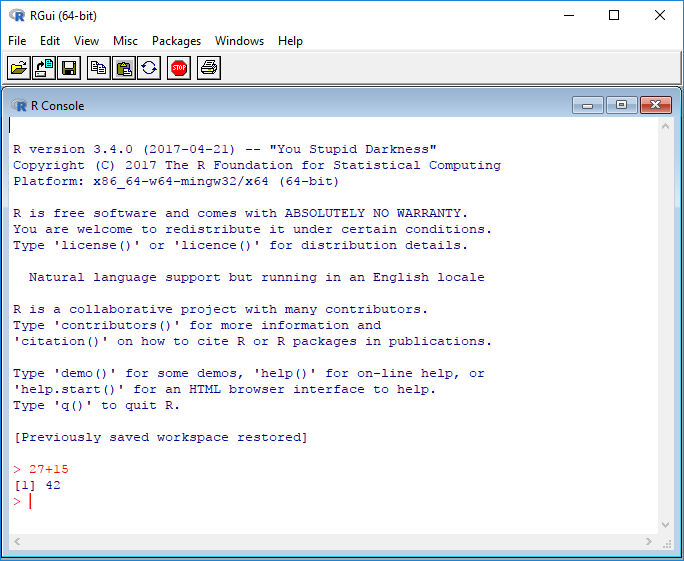
\includegraphics[width=.66\linewidth]{sss/rgui-win-42}
\vspace{\baselineskip}
\end{center}

Mi recomendación es usar RStudio, un IDE (\eng{integrated development environment}) que nos ayudará a trabajar mucho más cómodamente con R. RStudio incluye una consola, un editor de código con resaltado de sintaxis, explorador de objetos y una larga lista de cosas que puede que no entiendas aún, pero que seguro harán tu vida más fácil. Con toda seguridad se \emph{ve} mejor que RGui. Puedes descargar RStudio de \url{https://www.rstudio.com/}, y también es gratis (asegúrate de haber instalado R antes de instalar RStudio).

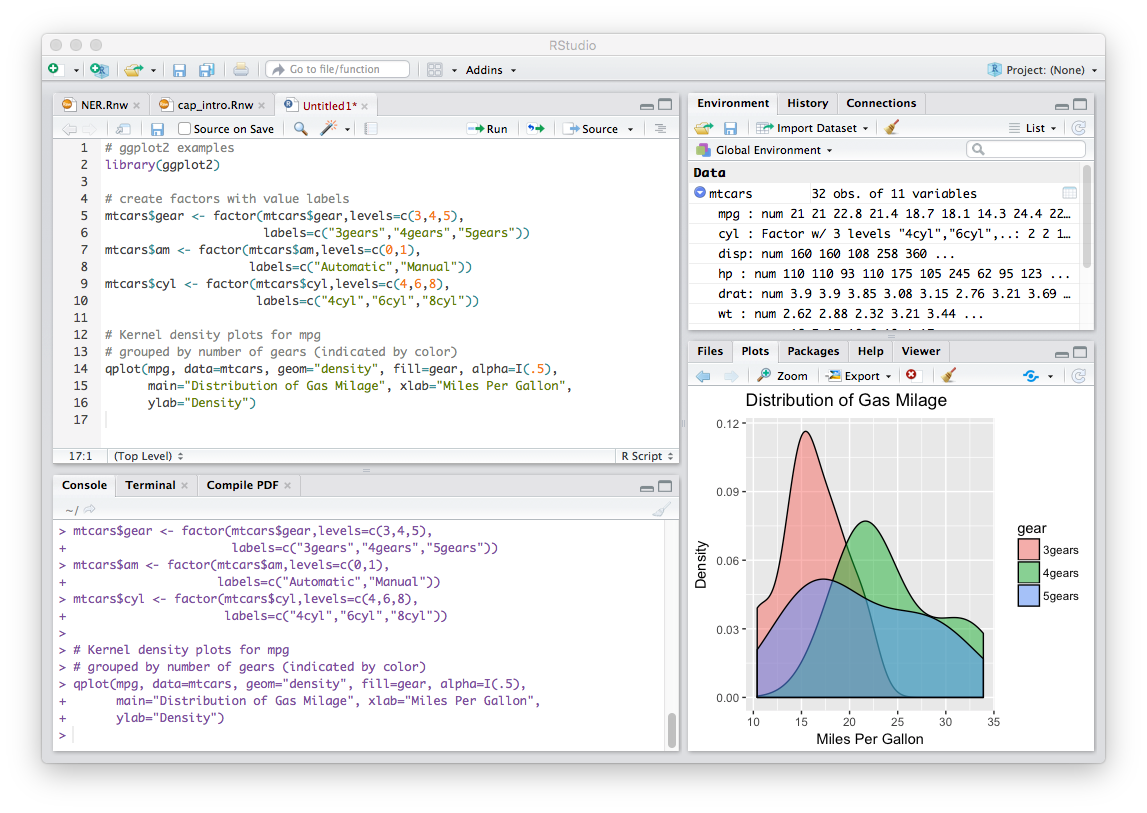
\includegraphics[width=\linewidth]{sss/rstudio-mac}

\subsection{Usar R interactivamente y a través de scripts}

\subsection{Trabajando con datos}

\subsubsection{Objetos y asignaciones}

R es un lenguaje interpretado, lo que significa que ejecuta nuestras instrucciones directamente, sin compilar un programa previo. Podemos usar R interactivamente a través de la consola:
\begin{knitrout}
\definecolor{shadecolor}{rgb}{0.969, 0.969, 0.969}\color{fgcolor}\begin{kframe}
\begin{alltt}
\hlnum{1}\hlopt{+}\hlnum{2}
\end{alltt}
\begin{verbatim}
## [1] 3
\end{verbatim}
\end{kframe}
\end{knitrout}

La mayoría de las operaciones y funciones en R no guardan el resultado de su ejecución. Por ejemplo, el resultado anterior (\verb|3|) es calculado pero no puede ser reutilizado sin volverse a calcular. Para lograr esto tenemos que asignar el resultado de la operación a un objeto:
\begin{knitrout}
\definecolor{shadecolor}{rgb}{0.969, 0.969, 0.969}\color{fgcolor}\begin{kframe}
\begin{alltt}
\hlstd{x} \hlkwb{<-} \hlnum{1}\hlopt{+}\hlnum{2}
\end{alltt}
\end{kframe}
\end{knitrout}

\section{R base vs. tidyverse}

Una de las críticas más comunes que se hace a R es que hay muchas (¿demasiadas?) maneras de lograr un mismo resultado. Por ejemplo, R base tiene un sistema propio para crear gráficos, pero también existe \paq{ggplot2} para lograr el mismo objetivo.
Esta multiplicidad de métodos puede hacer que R sea más difícil de aprender que lo necesario.

R es un lenguaje antiguo, y muchas de sus funcionalidades básicas ---lo que llamamos \kw{R base}--- operan bajo paradigmas anticuados. Uno de los más grandes aportes a la programación en R del útltimo tiempo fue realizado por Hadley Wickham, autor del \paq{tidyverse}. Este es un conjunto de paquetes que modernizan cómo usamos R para manipular datos, y están diseñados para trabajar bien entre ellos.

En un artículo para R-bloggers\footnote{\url{https://www.r-bloggers.com/teach-the-tidyverse-to-beginners/}}, David Robinson resume los dos principales ``curriculums'' de aprendizaje de R:
\begin{itemize}
\item \textbf{R base primero}: enseñar elementos de sintaxis como \verb|$| y \verb|[[]]|, loops, condicionales, tipos de datos y funciones base como \verb|tapply()|. Este enfoque no se concentra en un sólo marco de datos.
\item \textbf{tidyverse primero}: comenzar usando \paq{dplyr} para manipular marcos de datos y \paq{ggplot2} para crear gráficos. Luego introducir rápidamente el uso de \paq{tidyr} y \paq{purrr}. Usar el operador \verb|%>%| casi inmediatamente, pero dejar el uso de \verb|$| y \verb|[[]]| para más adelante. Este enfoque se concentra en un sólo marco de datos.
\end{itemize}

Mi opinión (y la de muchos otros) es que aprender a usar las herramientas del \paq{tidyverse} es más fácil y más productivo. La filosofía detrás del \paq{tidyverse} es similar a la de Python: "Debería haber una ---y preferiblemente sólo una--- forma obvia de lograr algo''. Esta filosofía es buena al aprender un lenguaje de programación, ya que entrega consistencia y evita confusiones.
Es por esto que en este documento prefiero usar herramientas del \paq{tidyverse} cada vez que sea posible.

Por ejemplo, en R base existen al menos tres formas de crear una variable nueva a partir de otra existente.
Por otro lado, con el \paq{tidyverse} hay una sóla forma de lograr esto, que además (a mi) me parece más legible:

\begin{knitrout}
\definecolor{shadecolor}{rgb}{0.969, 0.969, 0.969}\color{fgcolor}\begin{kframe}
\begin{alltt}
\hlcom{# Agregar una variable con R base}
\hlstd{mtcars}\hlopt{$}\hlstd{libras} \hlkwb{<-} \hlstd{mt}\hlopt{$}\hlstd{wt} \hlopt{*} \hlnum{1000}
\hlstd{mtcars[[}\hlstr{"libras"}\hlstd{]]} \hlkwb{<-} \hlstd{mtcars[[}\hlstr{"wt"}\hlstd{]]} \hlopt{/} \hlnum{1000}
\hlstd{mtcars[,} \hlstr{"libras"}\hlstd{]} \hlkwb{<-} \hlstd{mtcars[,} \hlstr{"wt"}\hlstd{]} \hlopt{/} \hlnum{1000}

\hlcom{# Agregar una variable con el tidyverse}
\hlstd{mtcars} \hlkwb{<-} \hlstd{mtcars} \hlopt \hlkwd{mutate}\hlstd{(}\hlkwc{libras} \hlstd{= wt} \hlopt{/} \hlnum{1000}\hlstd{)}
\end{alltt}
\end{kframe}
\end{knitrout}


Sin embargo, también hay elementos de R base que son importantes de aprender; de hecho, muchas cosas en R no son posibles sin ellos. Iremos introduciendo estos elementos a medida que nos sean útil para el tema en cuestión.

% Regresión lineal bivariada:



\chapter{Regresión lineal simple}



El modelo de regresión lineal es el caballo de batalla de la econometría aplicada.
Muchas de las preguntas que abordaremos comienzan con dos variables, digamos $x$ e $y$. Nos interesará entonces ``explicar $y$ en términos de $x$''.
Por ejemplo, $y$ podría ser la tasa de crímenes de varios barrios y $x$ el número de parques construidos en esos barrios.
O $y$ podría ser el porcentaje de los votos obtenidos por un partido y $x$ su gasto en la campaña electoral, etc.

Tomemos este último ejemplo y construyamos un caso concreto.
La \autoref{fig:votos_plot} muestra datos de 173 campañas entre los dos candidatos finalistas en elecciones de congreso estadounidenses.
Nos enfocamos en las variables de gasto y votos obtenidos por el ``candidato A'' (un nombre del que Kafka sin duda estaría orgulloso).
El eje $x$ corresponde al porcentaje gastado por este candidato (\verb|shareA|), mientras que el eje $y$ indica el porcentaje de los votos que obtuvo (\verb|voteA|).
El código para cargar los datos y crear el gráfico se muestra a continuación:

\begin{knitrout}
\definecolor{shadecolor}{rgb}{0.969, 0.969, 0.969}\color{fgcolor}\begin{kframe}
\begin{alltt}
\hlkwd{library}\hlstd{(tidyverse)}
\hlkwd{library}\hlstd{(haven)}
\hlstd{votos} \hlkwb{<-} \hlkwd{read_dta}\hlstd{(}\hlstr{"http://fmwww.bc.edu/ec-p/data/wooldridge/vote1.dta"}\hlstd{)}
\hlkwd{ggplot}\hlstd{(votos,} \hlkwd{aes}\hlstd{(shareA, voteA))} \hlopt{+} \hlkwd{geom_point}\hlstd{()}
\end{alltt}
\end{kframe}\begin{figure}[htb]

{\centering \includegraphics[width=4in,height=3in]{figs/votos_plot-1} 

}

\caption[Relación entre porcentaje de gasto (\texttt{shareA}) y porcentaje de votos obtenidos (\texttt{voteA})]{Relación entre porcentaje de gasto (\texttt{shareA}) y porcentaje de votos obtenidos (\texttt{voteA})}\label{fig:votos_plot}
\end{figure}


\end{knitrout}

\begin{Rbox}
\verb|library()| permite cargar paquetes de R, los que contienen más funciones y datos. \paq{haven} es un paquete que nos permite usar la función \verb|read_dta()| para leer una base de datos de Stata (con extensión \verb|*.dta|), y \paq{tidyverse} carga \paq{ggplot2}, un paquete que nos permite usar las funciones \verb|ggplot()| y \verb|geom_point()| para crear el gráfico de puntos.
\end{Rbox}

Al intentar modelar la relación entre $x$ e $y$ surgen una serie de preguntas. Quizás la más inmediata es: ``¿cuál es la relación funcional entre ambas variables?''
Nuestro primer supuesto será que las variables se relacionan de manera lineal, es decir,
\begin{equation}
y = ax + b.
\label{eq:ec_lin}
\end{equation}

La ecuación \eqref{eq:ec_lin} corresponde a la clásica función lineal de colegio, y su interpretación geométrica es la misma: $a$ es un término que representa la pendiente de una recta, y $b$ es su intercepto.
Este supuesto de relación lineal parece cumplirse bastante bien para nuestro ejemplo de la \autoref{fig:votos_plot}: no sabemos qué valores deberían tomar $a$ y $b$, pero definitivamente pareciera existir alguna combinación de valores de $a$ y $b$ tal que una línea se ajuste ``bien'' a los datos.

Sin embargo, el modelo expresado en \eqref{eq:ec_lin} asume que existe una relación lineal \emph{perfecta} entre $x$ e $y$, lo que es altamente restrictivo. 
En términos de la \autoref{fig:votos_plot}, es como suponer que podríamos trazar una recta que pasara por \emph{todos} los puntos, lo que evidentemente es imposible.
Entonces surge naturalmente la necesidad de permitir que otros factores ---distintos de $x$--- afecten en cierta medida a $y$, de forma que nuestro modelo tenga un margen de error.
Esto se logra agregando un \kw{término de error}, denotado por $\mu$, al modelo lineal.

Adicionalmente, por un simple tema de convención desde ahora en adelante llamaremos $\beta_0$ al parámetro del intercepto y $\beta_1$ al parámetro de la pendiente.
Entonces podemos reescribir nuestro modelo, que ahora es
\begin{equation}
y = \beta_0 + \beta_1x + \mu.
\label{eq:modelo_lineal_simple_poblacional}
\end{equation}
Esta ecuación define el \kw{modelo de regresión lineal simple}. Entendamos bien qué quiere decir cada palabra de este título:

\begin{itemize}
\item \textbf{modelo}, porque es un intento de simplificar la realidad para enfocarnos en algunos aspectos que nos interesan
\item \textbf{de}, una preposición en la gramática del español
\item \textbf{regresión} es el término usado originalmente por \textcite{galton_regression_1886}, aunque conceptualmente no guarda mucha relación con lo que hacemos ahora\footnote{\textcite{stigler_history_1986} cuenta una historia más detallada al respecto.} (pero el nombre es \eng{cool})
\item \textbf{lineal}, porque estamos asumiendo que los aspectos de la realidad que nos interesan ---las variables $x$ e $y$--- se relacionan de manera lineal en parámetros
\item \textbf{simple}, porque estamos restringiendo el análisis a solamente dos variables (por el momento).
\end{itemize}

Muchos libros tienen nombres distintos para $x$ e $y$. Yo uso la convención (bastante establecida) de referirme a $y$ como la \kw{variable dependiente} del modelo, y a $x$ como la \kw{variable independiente} del modelo. Estas son las variables que ya tenemos, y que intentaremos relacionar.
Ya mencionamos que $\mu$ es el llamado \kw{término de error}, que captura factores que afectan a $y$ que no hemos incluido en el modelo. Ojo que $\mu$ no es igual a $u$, y se pronuncia <<mu>>. Esto es sólo para enredar, claro.

En conjunto nos referiremos a $\beta_0$ y $\beta_1$ como los \kw{parámetros} (o coeficientes) del modelo.
Estos son simples números, pero como no los tenemos, intentaremos \emph{estimarlos}.
Encontrar una forma razonable de estimar estos parámetros será el objetivo de este capítulo (¡y más allá!).
Emprendemos esta tarea a continuación.

\section{Estimando los parámetros del modelo}

Nuestro objetivo ahora es estimar los parámetros $\beta_0$ y $\beta_1$ del modelo de regresión simple explicitado en \eqref{eq:modelo_lineal_simple_poblacional}. En términos geométricos, queremos encontrar una forma de estimar el intercepto y la pendiente de una recta para que esta se ajuste ``bien'' a los datos.

El modelo expresado en \eqref{eq:modelo_lineal_simple_poblacional} es nuestro supuesto de cómo se relacionan variables \emph{poblacionales}.
Sin embargo, nosotros (con alta probabilidad) no tendremos acceso a datos de la población completa, si no que a una \emph{muestra}.
Entonces tenemos que adaptar nuestra ecuación para que represente un \kw{modelo muestral}.
Logramos esto simplemente suponiendo que contamos con una muestra aleatoria de la población completa. Llamamos ${(x_i, y_i): i = 1, \ldots, n}$ a una muestra aleatoria de tamaño $n$ de la población, es decir, $x_i$ e $y_i$ son vectores con $n$ observaciones. Entonces reescribimos el modelo en términos de esta muestra:
\begin{equation}
y_i = \beta_0 + \beta_1 x_i + \mu_i,
\label{eq:modelo_lineal_simple}
\end{equation}
para todo $i$, donde $i = 1, \ldots, n$ es un índice que identifica a las observaciones (filas) en los datos.
Podríamos tener $n$ personas, familias o empresas en nuestra muestra.

La ecuación \eqref{eq:modelo_lineal_simple}, que sólo se diferencia de \eqref{eq:modelo_lineal_simple_poblacional} por ese pequeño subíndice $i$, es la versión \emph{muestral} del modelo lineal simple.
Como hemos supuesto que tenemos una muestra aleatoria, todavía podemos pensar que la variable dependiente $y_i$ es una función lineal de la variable independiente $x_i$, y que tenemos un término de error $\mu_i$ para capturar el efecto que otros factores tienen sobre $y_i$.
%Entonces intentaremos buscar ---o \emph{estimar}--- una combinación de parámetros $\beta_0$ y $\beta_1$ que se ajuste a los datos de nuestra muestra.

Por ejemplo, podríamos tener un vector $y_i$ con los salarios de $n=30$ personas, y modelarlo como una función lineal de los años de educación de esas personas, $x_i$. Resulta útil tener una base de datos concreta con estos vectores, por lo que usaremos una pequeña muestra de datos simulados.

\begin{knitrout}
\definecolor{shadecolor}{rgb}{0.969, 0.969, 0.969}\color{fgcolor}\begin{kframe}
\begin{alltt}
\hlcom{# Leer datos CSV de internet}
\hlstd{simdatos} \hlkwb{<-} \hlkwd{read_csv}\hlstd{(}
  \hlstr{"https://raw.githubusercontent.com/acarril/NER/master/datos/simdatos.csv"}\hlstd{)}
\hlcom{# Imprimir las primeras observaciones de los datos}
\hlstd{simdatos}
\end{alltt}
\begin{verbatim}
## # A tibble: 30 x 2
##        y         x
##    <int>     <dbl>
##  1     1  4.199913
##  2     1  7.510634
##  3     1  2.125473
##  4     2  8.988857
##  5     2 10.243105
##  6     2 11.296823
##  7     3  7.356365
##  8     3 10.505349
##  9     3 10.511601
## 10     4 12.434589
## # ... with 20 more rows
\end{verbatim}
\end{kframe}
\end{knitrout}

\begin{Rbox}
\verb|read_csv()| permite leer bases de datos en formato CSV. Lo usamos para leer una base en línea y luego asignamos esos datos al objeto \verb|simdatos| (datos simulados).
Luego escribimos el nombre del objeto (\verb|simdatos|) para imprimirlo. Como es un \eng{tibble} (una base de datos), R imprime solamente las primeras 10 observaciones.
Esto es útil para hacernos una idea rápida de las variables de la base y los valores que éstas toman.
\end{Rbox}

En estos datos la variable \verb|y| contiene salarios por hora (en miles de pesos) y la variable \verb|x| contiene años de educación.
Cada fila representa una observación (en este caso, una persona) distinta.
Siempre es recomendable graficar los datos, ya que un gráfico entrega mucha información y revela patrones que son difíciles de ver en los datos. Creamos un gráfico simple con \paq{ggplot2}:

\begin{knitrout}
\definecolor{shadecolor}{rgb}{0.969, 0.969, 0.969}\color{fgcolor}\begin{kframe}
\begin{alltt}
\hlkwd{ggplot}\hlstd{(simdatos,} \hlkwd{aes}\hlstd{(x, y))} \hlopt{+} \hlkwd{geom_point}\hlstd{()}
\end{alltt}
\end{kframe}

{\centering \includegraphics[width=4in,height=3in]{figs/unnamed-chunk-6-1} 

}



\end{knitrout}

\begin{Rbox}
\paq{ggplot2} es un paquete muy poderoso para crear gráficos de distintos tipos. Su principal función es \verb|ggplot()|, que permite definir los datos y las variables que usaremos (dentro de \verb|aes()|). Luego usamos \kw{funciones geom} para definir el tipo de gráfico; en este caso \verb|geom_point()| crea un gráfico de puntos.
\end{Rbox}

Vemos que existe una evidente relación lineal entre $x_i$ e $y_i$: a mayor nivel de educación parece haber mayor nivel de ingreso.
Esto es bueno para nosotros, ya que queremos ajustar los datos al modelo lineal que escribimos en \eqref{eq:modelo_lineal_simple}.
Cabe preguntarse ahora cuál es la manera óptima de elegir los parámetros que determinan dicha relación lineal, es decir, ¿cómo podemos elegir $\beta_0$ (el intercepto) y $\beta_1$ (la pendiente) para que nuestra predicción de $y_i$ sea lo mejor posible?

Es claro que podríamos elegir entre una infinita variedad de combinaciones de $\beta_0$ y $\beta_1$ para modelar los datos. Por ejemplo, el código de abajo simula 150 líneas con interceptos y pendientes ``razonables'', los que se grafican a continuación.

\begin{knitrout}
\definecolor{shadecolor}{rgb}{0.969, 0.969, 0.969}\color{fgcolor}\begin{kframe}
\begin{alltt}
\hlkwd{set.seed}\hlstd{(}\hlnum{314}\hlstd{)}
\hlstd{modelos} \hlkwb{<-} \hlkwd{tibble}\hlstd{(}
  \hlkwc{beta1} \hlstd{=} \hlkwd{runif}\hlstd{(}\hlnum{150}\hlstd{,} \hlopt{-}\hlnum{3}\hlstd{,} \hlnum{1}\hlstd{),}
  \hlkwc{beta2} \hlstd{=} \hlkwd{runif}\hlstd{(}\hlnum{150}\hlstd{,} \hlopt{-}\hlnum{1}\hlstd{,} \hlnum{1}\hlstd{)}
  \hlstd{)}
\hlkwd{ggplot}\hlstd{(simdatos,} \hlkwd{aes}\hlstd{(x, y))} \hlopt{+}
  \hlkwd{geom_point}\hlstd{()} \hlopt{+}
  \hlkwd{geom_abline}\hlstd{(}
    \hlkwd{aes}\hlstd{(}\hlkwc{intercept} \hlstd{= beta1,} \hlkwc{slope} \hlstd{= beta2),}
    \hlkwc{data} \hlstd{= modelos,} \hlkwc{alpha} \hlstd{=} \hlnum{1}\hlopt{/}\hlnum{4}
  \hlstd{)}
\end{alltt}
\end{kframe}

{\centering \includegraphics[width=4in,height=3in]{figs/unnamed-chunk-7-1} 

}



\end{knitrout}

Si bien hay muchas líneas que claramente no se ajustan bien a los datos, varias otras sí lo hacen, y resulta difícil determinar a simple vista cuál es ``la mejor'' (asumiendo que tal línea existe).
Es evidente que necesitamos un criterio riguroso para elegir los parámetros $\beta_0$ y $\beta_1$ de manera óptima.
Esto es lo que veremos a continuación.


\section{Mínimos Cuadrados Ordinarios}
\label{sec:MCO}

El método de Mínimos Cuadrados Ordinarios (MCO) es una respuesta directa a la pregunta que planteamos recién: ¿qué criterio conviene usar para elegir el modelo lineal que se ajuste ``mejor'' a los datos?
Intuitivamente, la idea es minimizar el error de ajuste entre los datos reales contenidos en $y_i$ y los datos predichos por nuestra elección de $\beta_0$ y $\beta_1$, que denotaremos con $\hat y_i$.
%Intuitivamente, la idea es minimizar el error de ajuste entre la predicción de $y_i$ definida por nuestra elección de $\beta_0$ y $\beta_1$, y los valores reales de $y_i$.

%Geométricamente, el método de MCO equivale a minimizar la distancia vertical entre los puntos y la recta definida por el modelo.

Ahora formalizaremos esta intuición, y para esto necesitamos introducir un poco de notación nueva.
Recordemos que estamos trabajando con \eqref{eq:modelo_lineal_simple}, que es la versión muestral del modelo lineal simple (reimpresa a continuación para comodidad del lector):
\begin{equation*}
y_i = \beta_0 + \beta_1 x_i + \mu_i.
\end{equation*}
Dada una muestra de datos, llamaremos $\hat\beta_0$ y $\hat\beta_1$ a nuestra estimación de los coeficientes.
Entonces la \kw{línea de regresión}, denotada por $\hat y_i$, está definida como
\begin{equation}
\hat y_i = \hat{\beta}_0 + \hat\beta_1 x_i.
\label{eq:linea_regresion}
\end{equation}
Algebraicamente, $\hat y_i$ es el vector que resulta de multiplicar el vector $x_i$ por el escalar $\hat\beta_1$ y luego sumarle $\hat\beta_0$.
Geométricamente, $\hat y_i$ es simplemente una recta que resulta de aplicar una transformación lineal a $x_i$, donde el intercepto y la pendiente dependen de los valores que hayamos elegido para $\hat\beta_0$ y $\hat\beta_1$ en \eqref{eq:linea_regresion}. La \autoref{fig:MCO} muestra una línea de regresión en azul.

\begin{knitrout}
\definecolor{shadecolor}{rgb}{0.969, 0.969, 0.969}\color{fgcolor}\begin{figure}[htb]

{\centering \includegraphics[width=4in,height=3in]{figs/MCO-1} 

}

\caption[Línea de regresión $\hat y_i$ en azul y residuo $\hat \mu_i$ en rojo]{Línea de regresión $\hat y_i$ en azul y residuo $\hat \mu_i$ en rojo}\label{fig:MCO}
\end{figure}


\end{knitrout}

Ahora, si tomamos la diferencia entre $y_i$ (los datos) y $\hat y_i$ (nuestra predicción) obtenemos $\hat\mu_i$, el \kw{residuo} de nuestra estimación:
\begin{align}
\hat \mu_i &= y_i - \hat y_i \notag \\
\hat \mu_i &= y_i - \hat\beta_0 + \hat\beta_1 x_i.
\label{eq:residuos}
\end{align}
Gráficamente el residuo corresponde a la distancia vertical entre cada punto (los datos $y_i$) y la recta (la predicción $\hat y_i$), dibujado con líneas rojas en la \autoref{fig:MCO}.
Es decir que para cada observación $i$ tenemos una medida de la magnitud del error que una elección particular de $\hat\beta_0$ y $\hat\beta_1$ producen.

Armados con esta notación podemos volver a la pregunta central: ¿Cómo elegimos de manera óptima los parámetros?
El método de MCO consiste en elegir $\hat\beta_0$ y $\hat\beta_1$ en \eqref{eq:residuos} tal que se minimice la suma de los residuos al cuadrado.\footnote{¿Por qué al cuadrado? Porque se asume que es irrelevante si el error es una subestimación o una sobreestimación, de forma que lo único que importa es la magnitud. ¿Por qué no se usa el valor absoluto entonces? Buena pregunta: \url{https://stats.stackexchange.com/q/46019/91358}. Básicamente, porque es algebraicamente más simple manejar valores cuadráticos, y no hace ninguna diferencia en el resultado final.}
Geométricamente esto es equivalente a minimizar la suma de las distancias verticales entre todos los puntos y la línea de regresión (las líneas rojas de la \autoref{fig:MCO}).
Matemáticamente el problema es
\begin{align}
\min_{\hat\beta_0,\hat\beta_1} & \sum_{i=1}^n \hat\mu_i^2 \notag \\
\Leftrightarrow \min_{\hat\beta_0,\hat\beta_1} & \sum_{i=1}^n (y_i - \hat\beta_0 - \hat\beta_1 x_i)^2.
\label{eq:prob_min_MCO}
\end{align}

Al resolver esta minimización obtendremos los estimadores MCO.\footnote{La derivación paso a paso puede encontrarse, por ejemplo, en \textcite[cap. 2]{wooldridge_introductory_2016}.}
Estos corresponden a la elección óptima de $\hat\beta_0$ y $\hat\beta_1$ que hemos estado buscando:
\begin{align}
\hat \beta_1 &= \sum_{i=1}^n \frac{\sum_{i=1}^n (x_i - \bar x)(y_i - \bar y)}{\sum_{i=1}^n (x_i - \bar x)^2} \notag \\
 &= \frac{\Cov (x,y)}{\Var(x)} \label{eq:MCO_beta1} \\
\hat \beta_0 &= \bar y - \hat\beta_1 \bar x, \label{eq:MCO_beta0}
\end{align}
donde $\bar x$ e $\bar y$ son los promedios de $x_i$ e $y_i$, $\Var(x)$ es la varianza muestral de $x$ y $\Cov(x,y)$ es la covarianza muestral de $x$ e $y$.

¡Hemos logrado nuestro objetivo!
Lo anterior significa que para encontrar los estimadores MCO y obtener la línea de regresión que mejor se ajuste a los datos solo tenemos que calcular cuatro cosas: $\bar y$, $\bar x$, $\Cov (x,y)$ y $\Var (x,y)$. ¡Hagámoslo ahora!

\begin{knitrout}
\definecolor{shadecolor}{rgb}{0.969, 0.969, 0.969}\color{fgcolor}\begin{kframe}
\begin{alltt}
\hlcom{# Indicar base de datos a usar}
\hlkwd{attach}\hlstd{(simdatos)}
\hlcom{# Promedios de 'x' e 'y'}
\hlstd{x.barra} \hlkwb{<-} \hlkwd{mean}\hlstd{(x)}
\hlstd{y.barra} \hlkwb{<-} \hlkwd{mean}\hlstd{(y)}
\hlcom{# Varianza de 'x' y covarianza entre 'x' e 'y'}
\hlstd{var.x} \hlkwb{<-} \hlkwd{var}\hlstd{(x)}
\hlstd{cov.xy} \hlkwb{<-} \hlkwd{cov}\hlstd{(x,y)}
\hlcom{# Calcular parámetros MCO}
\hlstd{beta1} \hlkwb{<-} \hlstd{cov.xy}\hlopt{/}\hlstd{var.x}
\hlstd{beta0} \hlkwb{<-} \hlstd{y.barra} \hlopt{-} \hlstd{beta1}\hlopt{*}\hlstd{x.barra}
\hlcom{# 'Desactivar' base de datos}
\hlkwd{detach}\hlstd{(simdatos)}
\hlcom{# Imprimir parámetros calculados}
\hlstd{beta0}
\end{alltt}
\begin{verbatim}
## [1] -1.185369
\end{verbatim}
\begin{alltt}
\hlstd{beta1}
\end{alltt}
\begin{verbatim}
## [1] 0.4311958
\end{verbatim}
\end{kframe}
\end{knitrout}

\begin{Rbox}
La función \verb|attach()| es útil para indicar que vamos a usar una base de datos en particular para todas las funciones que siguen. Entonces cuando calculamos el promedio de \verb|x| con \verb|mean(x)|, R sabe que se trata de la variable \verb|x| en el marco \verb|simdatos| (y no de \verb|votos|, por ejemplo). Luego usamos \verb|detach()| para ``desactivar'' el uso de la base que indicamos previamente.
\end{Rbox}

Vemos que es fácil calcular los estimadores MCO, y para este ejemplo particular obtuvimos que $\hat \beta_0 = -1.19$ y $\hat \beta_1 = 0.43$ (redondeando).
Con esto podemos completar la línea de regresión definida en \eqref{eq:linea_regresion}, usando nuestras estimaciones:
\begin{equation*}
\hat y_i = -1.19 + 0.43x_i.
\end{equation*}
Esto está bien, pero no es demasiado práctico para visualizar lo que hemos logrado.
Una alternativa mejor es usar estos parámetros para graficar $\hat y_i$ sobre los datos:

\begin{knitrout}
\definecolor{shadecolor}{rgb}{0.969, 0.969, 0.969}\color{fgcolor}\begin{kframe}
\begin{alltt}
\hlcom{# Graficar línea de regresión MCO}
\hlkwd{ggplot}\hlstd{(simdatos,} \hlkwd{aes}\hlstd{(x,y))} \hlopt{+}
  \hlkwd{expand_limits}\hlstd{(}\hlkwc{x} \hlstd{=} \hlnum{0}\hlstd{,} \hlkwc{y} \hlstd{=} \hlopt{-}\hlnum{2.5}\hlstd{)} \hlopt{+}
  \hlkwd{geom_point}\hlstd{()} \hlopt{+}
  \hlkwd{geom_abline}\hlstd{(}
    \hlkwc{intercept} \hlstd{= beta0,} \hlkwc{slope} \hlstd{= beta1,}
    \hlkwc{color} \hlstd{=} \hlstr{"blue"}\hlstd{,} \hlkwc{show.legend} \hlstd{=} \hlnum{FALSE} \hlstd{)}
\end{alltt}
\end{kframe}

{\centering \includegraphics[width=4in,height=3in]{figs/unnamed-chunk-9-1} 

}



\end{knitrout}

Finalmente, si bien resulta útil calcular explícitamente los estimadores para entender mejor qué es lo que estamos haciendo, esto no es demasiado práctico: estamos calculando y guardando promedios, varianzas y covarianzas que no nos interesan.
En realidad cualquier programa estadístico (decente) tiene algún método para estimar los parámetros de un modelo lineal de manera más compacta, y R no es la excepción:

\begin{knitrout}
\definecolor{shadecolor}{rgb}{0.969, 0.969, 0.969}\color{fgcolor}\begin{kframe}
\begin{alltt}
\hlcom{# Estimar directamente los parámetros de un modelo lineal}
\hlkwd{lm}\hlstd{(y} \hlopt{~} \hlstd{x,} \hlkwc{data} \hlstd{= simdatos)}
\end{alltt}
\begin{verbatim}
## 
## Call:
## lm(formula = y ~ x, data = simdatos)
## 
## Coefficients:
## (Intercept)            x  
##     -1.1854       0.4312
\end{verbatim}
\end{kframe}
\end{knitrout}

\begin{Rbox}
La función \verb|lm()| viene de \eng{linear model}, y permite calcular rápidamente los parámetros de un modelo lineal. El primer argumento de la función es una fórmula de R, que no es exactamente lo mismo que una fórmula en el sentido usual de la palabra. Por el momento basta entender que a la izquierda de \verb|~| indicamos la variable dependiente, mientras que a la derecha indicamos las variables independientes. Entonces \verb|lm()| toma una fórmula como \verb|y~x| y la traduce automáticamente a algo como \verb|y = beta0 + beta1 * x|.
\end{Rbox}

%Una de las ventajas de usar \verb|lm()| es que podemos guardar sus resultados en un objeto, el que luego podemos manipular para extraer otro tipo de información útil del modelo. A continuación veremos cómo extraer, manipular e interpretar esta información, lo que nos dará una comprensión mucho más profunda de lo que estamos haciendo.

Hemos calculado los parámetros del modelo, y sabemos lo que éstos quieren decir en términos matemáticos (minimizan el la suma de los errores cuadráticos) y geométricos (son el intercepto y la pendiente de la línea de ``mejor'' ajuste).
¿Pero pueden decirnos algo de los datos que usamos para calcularlos?
¿Qué significa, en términos de la relación entre educación e ingreso, que $\hat \beta_0 = -1.19$ y $\hat \beta_1 = 0.43$?
Saber interpretar correctamente los parámetros de una regresión es un arte, y comenzamos a explorarlo a continuación.


\section{Interpretando los parámetros estimados}

Una vez obtenidos los parámetros del modelo, nos interesa poder interpretarlos de manera útil. ¿Qué es lo que quiere decir que hayamos obtenido ciertos valores de $\hat\beta_0$ y $\hat\beta_1$, más allá de ser el intercepto y la pendiente de una ecuación?
Para explorar este tema dejaremos de usar datos simulados y pasaremos a datos reales.
En particular usaremos \verb|wage2|, que es una de las bases usadas en \textcite{wooldridge_introductory_2016} y contiene información de años de educación e ingresos para 935 personas.\footnote{Esta base es un subconjunto de los datos del estudio de \textcite{blackburn_unobserved_1992}.}

\begin{knitrout}
\definecolor{shadecolor}{rgb}{0.969, 0.969, 0.969}\color{fgcolor}\begin{kframe}
\begin{alltt}
\hlstd{ingresos} \hlkwb{<-} \hlkwd{read_dta}\hlstd{(}\hlstr{"http://fmwww.bc.edu/ec-p/data/wooldridge/wage2.dta"}\hlstd{)}
\hlstd{ingresos} \hlkwb{<-} \hlkwd{select}\hlstd{(ingresos, wage, educ)}
\end{alltt}
\end{kframe}
\end{knitrout}

\begin{Rbox}
Usamos \verb|haven::read_dta()| para leer bases de datos de Stata, como ya hicimos previamente. En la segunda línea, \verb|select()| nos permite seleccionar las variables \verb|wage| y \verb|educ| de la base \verb|ingresos| que acabamos de leer. Asignamos el resultado de \verb|select()| al mismo objeto para sobreescribirlo con solamente las variables que nos interesan.
\end{Rbox}

Sólo por conveniencia, podemos escribir la línea de regresión definida en \eqref{eq:linea_regresion} usando los nombres de las variables que nos interesan: salario mensual en dólares (\verb|wage|) y años de educación (\verb|educ|). Luego estimamos los coeficientes del modelo con \verb|lm()|, esta vez definiendo una fórmula donde \verb|wage| es la variable dependiente y \verb|educ| es la variable independiente:
\begin{align*}
\hat y &= \hat\beta_0 + \hat\beta_1 x \\
\Longleftrightarrow \widehat{wage} &= \hat\beta_0 + \hat\beta_1 {educ}.
\end{align*}

\begin{knitrout}
\definecolor{shadecolor}{rgb}{0.969, 0.969, 0.969}\color{fgcolor}\begin{kframe}
\begin{alltt}
\hlkwd{lm}\hlstd{(wage} \hlopt{~} \hlstd{educ,} \hlkwc{data} \hlstd{= ingresos)}
\end{alltt}
\begin{verbatim}
## 
## Call:
## lm(formula = wage ~ educ, data = ingresos)
## 
## Coefficients:
## (Intercept)         educ  
##      146.95        60.21
\end{verbatim}
\begin{alltt}
\hlkwd{ggplot}\hlstd{(ingresos,} \hlkwd{aes}\hlstd{(educ, wage))} \hlopt{+}
  \hlkwd{geom_point}\hlstd{()} \hlopt{+}
  \hlkwd{geom_smooth}\hlstd{(}\hlkwc{method} \hlstd{=} \hlstr{"lm"}\hlstd{,} \hlkwc{se} \hlstd{=} \hlnum{FALSE}\hlstd{)}
\end{alltt}
\end{kframe}\begin{figure}[htb]

{\centering \includegraphics[width=4in,height=3in]{figs/ingresos_lm-1} 

}

\caption[Modelo de regresión lineal relacionando años de educación (\texttt{educ}) y salario (\texttt{wage})]{Modelo de regresión lineal relacionando años de educación (\texttt{educ}) y salario (\texttt{wage})}\label{fig:ingresos_lm}
\end{figure}


\end{knitrout}
\begin{Rbox}
\verb|geom_smooth| es una función geom que podemos usar en conjunto con \verb|ggplot()| para graficar medias condicionales. Al usar la opción \verb|method = "lm"| indicamos que queremos graficar un modelo lineal entre las variables de los ejes. El uso de \verb|se=FALSE| es para desactivar los intervalos de confianza, tema del que hablaremos más adelante.
\end{Rbox}

El intercepto del modelo lineal ($\beta_0$) es el valor predicho de $y$ cuando $x=0$. En términos de nuestro ejemplo, si una persona tiene 0 años de educación el modelo predice un ingreso mensual promedio de 146.95 dólares.
Es importante notar que en algunos contextos no tiene demasiado sentido pensar en $x=0$ (¿cuántas personas con 0 años de educación existirán? ¿cuántas hay en los datos?). En esas situaciones $\hat\beta_0$ no tiene mucho valor en sí mismo, y es labor del investigador discriminar los casos dónde esto ocurra.
Exploraremos este punto con mayor profundidad en otro ejemplo más adelante.

El coeficiente estimado para la pendiente ($\hat\beta_1$) nos dice la cantidad en la que cambia $\hat y$ cuando $x$ aumenta en una unidad. En otras palabras,
\begin{equation}
\Delta \hat y = \hat \beta_1 \cdot \Delta x,
\end{equation}
donde el operador $\Delta$ (``delta'') significa simplemente ``el cambio en ...''.

El aumento de $x$ puede ir asociado tanto a un aumento como a una disminución de $\hat y$.
Si $\hat\beta_1 > 0$ entonces un aumento de una unidad de $x$ está asociado a un aumento de $\hat\beta_1$ en $\hat y$; si $\hat\beta_1 < 0$ entonces un aumento de una unidad de $x$ está asociado a una disminución de $-\hat\beta_1$ en $\hat y$.
Por ejemplo, en la estimación graficada en la \autoref{fig:ingresos_lm} hemos obtenido que $\hat\beta_1 = 60.21$.
Esto puede interpretarse como que un aumento de un año de educación ($x$ aumenta en una unidad) está asociado a un aumento promedio de (casi) 60 dólares en el salario.
Podemos asegurar que un aumento de $x$ se relaciona con un aumento en $\hat y$ porque el signo del coeficiente estimado es positivo; si el coeficiente estimado hubiese sido negativo, entonces diríamos que un año adicional de educación \emph{reduce} el salario promedio (¿tendría sentido esto?).

Hemos sido cuidadosos en no atribuirle una interpretación causal a la variable independiente. En otras palabras, evitamos decir que un año adicional de educación \emph{provoca} un aumento promedio de 60 dólares en el ingreso. La pregunta de causalidad es importante, y un tema muy estudiado en econometría. Sin embargo, sólo podremos hablar de causalidad más adelante, cuando hayamos estudiado las propiedades estadísticas de los estimadores de MCO e impongamos supuestos más fuertes sobre la población.

\subsection{La unidad de medida}

Habrás notado que la unidad de medida de las variables es clave a la hora de interpretar los coeficientes estimados. En el ejemplo anterior $x$ son años de educación, y por lo tanto $\hat\beta_1 = 60.21$ implica que un año adicional de educación está asociado a un aumento de 60.21 dólares en el salario mensual promedio, porque la unidad de $y$ son dólares mensuales.

Veamos ahora cómo cambian los parámetros estimados cuando cambia la unidad de medida de las variables.
En concreto, usaremos los datos \verb|mtcars|, que contiene 32 observaciones de modelos de auto.
Nos concentramos en una variable que indica su rendimiento en millas por galón (\verb|mpg|) y otra con su peso en miles de libras (\verb|wt|).

\begin{knitrout}
\definecolor{shadecolor}{rgb}{0.969, 0.969, 0.969}\color{fgcolor}\begin{kframe}
\begin{alltt}
\hlcom{# Calcular estadística descriptiva para las variables 'mpg' y 'wt'}
\hlkwd{summary}\hlstd{(}\hlkwd{select}\hlstd{(mtcars, mpg, wt))}
\end{alltt}
\begin{verbatim}
##       mpg              wt       
##  Min.   :10.40   Min.   :1.513  
##  1st Qu.:15.43   1st Qu.:2.581  
##  Median :19.20   Median :3.325  
##  Mean   :20.09   Mean   :3.217  
##  3rd Qu.:22.80   3rd Qu.:3.610  
##  Max.   :33.90   Max.   :5.424
\end{verbatim}
\begin{alltt}
\hlcom{# Estimar el modelo lineal }
\hlkwd{lm}\hlstd{(mpg} \hlopt{~} \hlstd{wt,} \hlkwc{data} \hlstd{= mtcars)}
\end{alltt}
\begin{verbatim}
## 
## Call:
## lm(formula = mpg ~ wt, data = mtcars)
## 
## Coefficients:
## (Intercept)           wt  
##      37.285       -5.344
\end{verbatim}
\end{kframe}
\end{knitrout}




\begin{Rbox}
\verb|summary()| es una de las funciones más útiles de R base, ya que permite producir un resumen con información útil de distintos objetos: bases de datos, modelos, etc. En este caso la usamos para producir estadística descriptiva de las variables elegidas con \verb|select()|, para evitar usar la función sobre todas las variables de \verb|mtcars|.
\end{Rbox}

Al estimar este modelo obtenemos que $\hat\beta_1 = -5.34$. Esto significa que un aumento de una unidad en \verb|wt| está asociado a una disminución promedio de $5.34$ en \verb|mpg|.

OK, ¿y?

Como no sé mucho de autos ni del sistema métrico imperial, no tengo idea si esto es mucho o poco.
A pesar que entiendo cómo interpretar el coeficiente en términos algebraicos, la unidad de medida de las variables hace que esta información no sea tan útil (para mi).

Afortunadamente es muy fácil transformar las variables y luego volver a estimar el modelo con ellas. Crearemos las variables \verb|rendimiento_kml| con el rendimiento en kilómetros por litro y \verb|peso_kg| con el peso en kilógramos de cada auto:

\begin{knitrout}
\definecolor{shadecolor}{rgb}{0.969, 0.969, 0.969}\color{fgcolor}\begin{kframe}
\begin{alltt}
\hlcom{# Crear marco 'autos' con las variables que nos interesan}
\hlstd{autos} \hlkwb{<-} \hlkwd{as_tibble}\hlstd{(}\hlkwd{select}\hlstd{(}\hlkwd{rownames_to_column}\hlstd{(mtcars,} \hlkwc{var} \hlstd{=} \hlstr{"modelo"}\hlstd{),}
                          \hlstd{modelo, mpg, wt))}
\hlcom{# Crear dos variables nuevas de rendimiento y peso}
\hlstd{autos} \hlkwb{<-} \hlkwd{mutate}\hlstd{(autos,}
                \hlkwc{rendimiento_kml} \hlstd{=  mpg} \hlopt{*} \hlnum{0.425144}\hlstd{,}
                \hlkwc{peso_kg} \hlstd{= wt} \hlopt{*} \hlnum{453.592}\hlstd{)}
\hlcom{# Estimar el modelo con estas nuevas variables}
\hlkwd{lm}\hlstd{(rendimiento_kml} \hlopt{~} \hlstd{peso_kg,} \hlkwc{data} \hlstd{= autos)}
\end{alltt}
\begin{verbatim}
## 
## Call:
## lm(formula = rendimiento_kml ~ peso_kg, data = autos)
## 
## Coefficients:
## (Intercept)      peso_kg  
##   15.851548    -0.005009
\end{verbatim}
\end{kframe}
\end{knitrout}


Esta transformación todavía presenta un pequeño problema. Como la unidad de medida de \verb|peso_kg| son kilos, $\hat\beta_1 = -0.005$ nos dice que por cada kilo adicional el modelo predice una reducción de 0.005 en el rendimiento promedio.
Claramente pensar en un kilo adicional en algo tan pesado como un auto no tiene mucho sentido, por lo que estimaremos el modelo con una variable que indique el peso en unidades de 100 kilos:
\begin{knitrout}
\definecolor{shadecolor}{rgb}{0.969, 0.969, 0.969}\color{fgcolor}\begin{kframe}
\begin{alltt}
\hlcom{# Agregar variable con peso en unidades de 100kg}
\hlstd{autos} \hlkwb{<-} \hlstd{autos} \hlopt \hlkwd{mutate}\hlstd{(}\hlkwc{peso_100kg} \hlstd{= peso_kg} \hlopt{/} \hlnum{100}\hlstd{)}
\hlcom{# Estimar modelo con esta nueva variable independiente}
\hlkwd{lm}\hlstd{(rendimiento_kml} \hlopt{~} \hlstd{peso_100kg,} \hlkwc{data} \hlstd{= autos)}
\end{alltt}
\begin{verbatim}
## 
## Call:
## lm(formula = rendimiento_kml ~ peso_100kg, data = autos)
## 
## Coefficients:
## (Intercept)   peso_100kg  
##     15.8515      -0.5009
\end{verbatim}
\end{kframe}
\end{knitrout}


\begin{Rbox}
Este bloque introduce el uso del \kw{operador de pipa}, \verb|%>%|.
Creado por Milton Bache en su paquete \paq{magrittr}, el operador de pipa sirve para pasar un objeto como primer argumento de una función.
Entonces en lugar de escribir \verb|f(x,y)| podemos escribir de manera equivalente \verb|x %>% f(y)|.
Esto permite ``desanidar'' funciones, ya que el operador es recursivo: operaciones como $f(g(x))$ pueden expresarse como \verb|x %>% g %>% f|, lo que las hace más legibles.
\end{Rbox}

Ahora podemos interpretar el modelo más fácilmente, teniendo unidades adecuadas.
El coeficiente asociado a la variable independiente se puede interpretar como que el modelo predice una reducción promedio de $0.5$ km/l por cada 100 kilos adicionales que pese un auto.
Esto definitivamente parece razonable, y los coeficientes entregan información útil directamente.
Es importante notar que este valor de $\hat\beta_1$ usando \verb|peso_100kg| es igual al calculado usando \verb|peso_kg|, pero multiplicado por 100. Al realizar una transformación lineal sobre la variable, transformamos de manera inversa el coeficiente asociado.

Por otro lado, el parámetro del intercepto indica que el modelo predice un rendimiento promedio de $15.85$ para un auto de 0 kilos.
Este corresponde a un claro caso donde el intercepto no tiene sentido en sí mismo, ya que es imposible un auto de 0 kilos.

Recordemos que la línea de regresión de este modelo es
\begin{equation*}
\hat y_i = 15.85 -0.5 \cdot x_i.
\end{equation*}
Podemos usar la ecuación de la línea de regresión para calcular el valor predicho $\hat y_i$ dado un nivel de $x_i$. Por ejemplo, nuestra estimación predice que un auto de 1600 kilos tendrá un rendimiento promedio de $15.85 -0.5 \cdot 16 = 7.84$ km/l.
Esto se ajusta bastante a los datos reales, como puede apreciarse en la \autoref{fig:autos_lm}.
%Como siempre, es conveniente dibujar esta línea $\hat y_i$ sobre los datos. El gráfico se muestra en la \autoref{fig:autos_lm}.

\begin{knitrout}
\definecolor{shadecolor}{rgb}{0.969, 0.969, 0.969}\color{fgcolor}\begin{kframe}
\begin{alltt}
\hlcom{# Graficar la línea de regresión sobre los datos}
\hlstd{autos} \hlopt \hlkwd{ggplot}\hlstd{(}\hlkwd{aes}\hlstd{(peso_100kg, rendimiento_kml))} \hlopt{+}
  \hlkwd{geom_point}\hlstd{()} \hlopt{+}
  \hlkwd{geom_smooth}\hlstd{(}\hlkwc{method} \hlstd{=} \hlstr{"lm"}\hlstd{,} \hlkwc{se} \hlstd{=} \hlnum{FALSE}\hlstd{)}
\end{alltt}
\end{kframe}\begin{figure}[htb]

{\centering \includegraphics[width=4in,height=3in]{figs/autos_lm-1} 

}

\caption[Modelo de regresión lineal relacionando el peso de un auto (en unidades de 100 kilos) y su rendimiento (en kilómetros por litro)]{Modelo de regresión lineal relacionando el peso de un auto (en unidades de 100 kilos) y su rendimiento (en kilómetros por litro)}\label{fig:autos_lm}
\end{figure}


\end{knitrout}



%\subsubsection{Errores estándar de los coeficientes}

%Los parámetros estimados ---los coeficientes de MCO, en este caso--- son estadísticos muestrales que usamos para hacer inferencias de los parámetros poblacionales. Es importante tener en cuenta que son estos parámetros poblacionales los que nos interesan en realidad, pero como no podemos observarlos directamente, debemos inferirlos por medio de una muestra finita.

%Es evidente que si tomáramos una muestra distinta a la actual, lo más probable es que estimaríamos parámetros diferentes. Si tomaras datos de otras 935 personas (o cualquier número, en realidad) es muy posible que al aplicar el mismo modelo obtuviéramos valores de $\beta_0$ y $\beta_1$ distintos de coefficients(modelo)[1] y coefficients(modelo)[2]. Además es muy probable que nuevamente ninguno de los dos sea igual al verdadero parámetro poblacional, que es el que nos interesa. Si continuáramos este proceso de tomar diferentes muestras y estimar los mismos parámetros una y otra vez, veríamos que la frecuencia relativa de las estimaciones obtenidas sigue una distribución de probabilidad, y por el Teorema Central del Límite sabemos que es probable que esta distribución sea normal. Entonces es importante para nuestra estimación que cuantifiquemos la cantidad de incertidumbre en esta distribución poblacional desconocida. Ahí es donde entra el concepto de error estándar, que corresponde a nuestra estimación de la desviación estándar de la distribución de estos muestreos. En términos intuitivos, es una medida de la incertidumbre de $\hat\beta$.

%Encerramos \verb|lm()| dentro de \verb|summary()| para obtener información más detallada de las estimaciones del modelo, incluyendo estimaciones para los errores estándar de los coeficientes:

%<<>>=
%summary(lm(wage ~ educ, data = ingresos))
%@

%todo: explicar mejor todos los summary de ols

%<<>>=
%ggplot(ingresos, aes(educ, wage)) + 
%  geom_point() + 
%  geom_smooth(method = "lm")
%@

\section{Distribución muestral de los estimadores}
\label{sec:distribucion_estimadores}

Es importante tener en cuenta que los estimadores MCO son eso: estimadores de un parámetro poblacional real.
Podemos pensar en MCO como una máquina en donde entra una muestra y salen estimadores, tal como se representa en la \autoref{fig:MCOcaja}.
Las estimaciones que realicemos dependen de la muestra que usemos, de forma que distintas muestran producirán distintas estimaciones de los parámetros.

%<<>>=
%library(hdm)
%AJR <- as_tibble(AJR)
%lm(GDP ~ logMort, data = AJR)
%ggplot(AJR, aes(logMort, GDP)) + geom_point() + geom_smooth(method = "lm")
%@

% Sacado de http://www.mattblackwell.org/
%\includegraphics[width=\textwidth]{figs/ols_blackbox}

\begin{figure}[htb]
\centering
\begin{tikzpicture}[thick]

\path [every node/.style={inner sep=0.2cm, outer sep=0.2cm}]
  node[anchor=east] (muestra1) at (0, 1.6cm) {Muestra 1: $\{ (y_1,x_1),\ldots,(y_n,x_n) \}$}
  node[anchor=east] (muestra2) at (0, 0.8cm) {Muestra 2: $\{ (y_1,x_1),\ldots,(y_n,x_n) \}$}
  node (muestradots) at (-4,0) {$\vdots$}
  node[anchor=east] (muestrak-1) at (0, -0.8cm) {Muestra $k-1$: $\{ (y_1,x_1),\ldots,(y_n,x_n) \}$}
  node[anchor=east] (muestrak) at (0, -1.6cm) {Muestra $k$: $\{ (y_1,x_1),\ldots,(y_n,x_n) \}$}
  [xshift=3cm]
  node[draw, minimum width=3cm, minimum height=3cm, anchor=center] (MCO) at (0,0) {MCO}
  [xshift=3cm]
  node[anchor=west] (est1) at (0, 1.6cm) {$(\hat\beta_0, \hat\beta_1)_{1}$}
  node[anchor=west] (est2) at (0, 0.8cm) {$(\hat\beta_0, \hat\beta_1)_{2}$}
  node[anchor=west] (estdots) at (1.15,0) {$\vdots$}
  node[anchor=west] (estk-1) at (0, -0.8cm) {$(\hat\beta_0, \hat\beta_1)_{k-1}$}
  node[anchor=west] (estk) at (0, -1.6cm) {$(\hat\beta_0, \hat\beta_1)_{k}$};

\begin{scope}[->,>=latex]
	% Entrada arriba
	\draw[->] (muestra1.east) to [out=0,in=140] ([yshift=1cm]MCO.west) ;
	\draw[->] (muestra2.east) to [out=0,in=140] ([yshift=.4cm]MCO.west) ;
	% Entrada abajo
	\draw[->] (muestrak-1.east) to [out=0,in=-140] ([yshift=-.4cm]MCO.west) ;
	\draw[->] (muestrak.east) to [out=0,in=-140] ([yshift=-1cm]MCO.west) ;
	% Salida arriba
	\draw[->] ([yshift=1cm]MCO.east) to [out=40,in=180] (est1.west) ;
	\draw[->] ([yshift=.4cm]MCO.east) to [out=40,in=180] (est2.west) ;
	% Salida abajo
	\draw[->] ([yshift=-.4cm]MCO.east) to [out=-40,in=-180] (estk-1.west) ;
	\draw[->] ([yshift=-1cm]MCO.east) to [out=-40,in=-180] (estk.west) ;
\end{scope}

\end{tikzpicture}
\caption{MCO es como una caja donde entran muestras y salen parámetros estimados}
\label{fig:MCOcaja}
\end{figure}

No es necesario creer en mi palabra. A continuación simulamos 500 muestreos aleatorios de 1000 observaciones cada uno. Nos concentraremos únicamente en el parámetro de la pendiente, $\beta_1$. Fijamos el verdadero valor de dicho parámetro en $\beta_1=0.7$ (en el código \verb|b <- 0.7|). Al simular los datos tomados de una población normal, usando los parámetros que hemos definido, estimamos el parámetro $k$ veces y obtenemos $k$ valores para $\hat\beta_1$, los que vamos guardando en el vector \verb|beta1|. Finalmente hacemos un gráfico de densidad con los valores de dicho vector.

% Simulacion de http://www.unc.edu/~carsey/teaching/ICPSR-2011/Sim%20Slides%20Handout.pdf
\begin{knitrout}
\definecolor{shadecolor}{rgb}{0.969, 0.969, 0.969}\color{fgcolor}\begin{kframe}
\begin{alltt}
\hlkwd{set.seed}\hlstd{(}\hlnum{1102}\hlstd{)} \hlcom{# fijar la semilla para resultados replicables}

\hlcom{# Parámetros poblacionales ("verdaderos")}
\hlstd{a} \hlkwb{<-} \hlnum{0.2} \hlcom{# verdadero valor del intercepto}
\hlstd{b} \hlkwb{<-} \hlnum{0.7} \hlcom{# verdadero valor de la pendiente}

\hlcom{# Parámetros de la simulación}
\hlstd{k} \hlkwb{<-} \hlnum{500} \hlcom{# número de simulaciones }
\hlstd{n} \hlkwb{<-} \hlnum{1000} \hlcom{# tamaño muestral}

\hlcom{# Comenzar simulación}
\hlstd{beta1} \hlkwb{<-} \hlkwd{numeric}\hlstd{(}\hlkwc{length} \hlstd{= k)} \hlcom{# vector vacío para guardar pendientes estimadas}
\hlkwa{for}\hlstd{(i} \hlkwa{in} \hlnum{1}\hlopt{:}\hlstd{k) \{} \hlcom{# loop de 500 simulaciones}
  \hlstd{x} \hlkwb{<-} \hlkwd{rnorm}\hlstd{(n,} \hlkwc{mean}\hlstd{=}\hlnum{2}\hlstd{,} \hlkwc{sd}\hlstd{=}\hlnum{1}\hlstd{)} \hlcom{# variable independiente}
  \hlstd{u} \hlkwb{<-} \hlkwd{rnorm}\hlstd{(n,} \hlkwc{mean}\hlstd{=}\hlnum{0}\hlstd{,} \hlkwc{sd}\hlstd{=}\hlnum{1}\hlstd{)} \hlcom{# término de error}
  \hlstd{y} \hlkwb{<-} \hlstd{a} \hlopt{+} \hlstd{b}\hlopt{*}\hlstd{x} \hlopt{+} \hlstd{u} \hlcom{# variable dependiente}
  \hlstd{estimacion} \hlkwb{<-} \hlkwd{lm}\hlstd{(y} \hlopt{~} \hlstd{x)} \hlcom{# estimar parámetros por MCO}
  \hlstd{beta1[i]} \hlkwb{<-} \hlkwd{coef}\hlstd{(estimacion)[}\hlnum{2}\hlstd{]} \hlcom{# guardar pendiente (2do coef) estimada}
\hlstd{\}}

\hlcom{# Graficar densidad de 500 pendientes estimadas}
\hlkwd{ggplot}\hlstd{(}\hlkwd{tibble}\hlstd{(beta1),} \hlkwd{aes}\hlstd{(beta1))} \hlopt{+}
  \hlkwd{geom_vline}\hlstd{(}\hlkwc{xintercept} \hlstd{= b,} \hlkwc{color} \hlstd{=} \hlstr{"forestgreen"}\hlstd{)} \hlopt{+}
  \hlkwd{geom_density}\hlstd{()}
\end{alltt}
\end{kframe}

{\centering \includegraphics[width=4in,height=3in]{figs/unnamed-chunk-18-1} 

}



\end{knitrout}

Lo que este gráfico nos muestra es que a pesar de que existe un único valor poblacional para uno de los parámetros estimados ($\beta_1$ en este caso), al estimar una regresión por MCO con distintas muestras obtendremos distintos valores estimados para dicho parámetro.
En un caso real no conoceremos el valor poblacional del parámetro, ni podremos tomar 500 muestras distintas... ¡tendremos suerte si obtenemos 1 buena muestra! Por eso, es esencial tener presente esta distribución de $\hat\beta$ al estimar un modelo.

Habrás notado que al tomar 500 muestras y estimar $\hat\beta_1$, los valores estimados se concentran en torno al verdadero valor de $\beta_1$, que es 0.7 en este ejemplo. ¡Esto es bueno... y no es casualidad! En realidad es una propiedad de los estimadores MCO.
A continuación formalizaremos esta y otras propiedades, con el fin de entender qué debe ocurrir para que se cumplan.

\section{Propiedades de los estimadores MCO}

Hasta ahora hemos aprendido a calcular e interpretar los parámetros de un modelo lineal simple.
%En la \autoref{sec:distribucion_estimadores} enfatizamos que nuestra estimación de $\hat\beta_0$ y $\hat\beta_1$ proviene de una distribución, ya que depende de la muestra con la que trabajemos.
%Entendemos entonces a $\hat\beta_0$ y $\hat\beta_1$ como estimadores de los verdaderos parámetros poblacionales, $\beta_0$ y $\beta_1$.
%Con esto en mente estudiaremos las propiedades de la distribución de $\hat\beta_0$ y $\hat\beta_1$ bajo distintas muestras aleatorias.
En la \autoref{sec:distribucion_estimadores} enfatizamos que los estimadores MCO ($\hat\beta_0$ y $\hat\beta_1$, o en general $\hat\beta$) tienen una distribución de probabilidad.
Intuitivamente, la razón por la que esto ocurre es porque nuestra estimación de $\hat\beta_0$ y $\hat\beta_1$ depende de la muestra aleatoria particular que tengamos de la población; si tomáramos distintas muestras, obtendríamos distintos valores para $\hat\beta$.
Entonces nuestra estimación de $\hat\beta$ es solo una realización de infinidad de posibilidades, como se muestra en la \autoref{fig:parametros_distribucion}.

\begin{figure}[htb]
  \centering
  \begin{tikzpicture}
    \begin{axis}[
    no markers, domain=0:8, samples=100,
    axis lines*=left, xlabel=, ylabel=$f(\hat\beta)$,
    every axis y label/.style={at=(current axis.above origin),anchor=south},
    every axis x label/.style={at=(current axis.right of origin),anchor=west},
    height=2.4in, width=3.2in,
    xtick={3},
    xticklabels={$\hat\beta$},
    ytick=\empty,
    enlargelimits=false, clip=false, axis on top,
    grid = major
    ]
    \addplot [very thick, black] {gauss(4,1)};
    \end{axis}
  \end{tikzpicture}
  \caption{La realización de $\hat\beta$ que nosotros observamos proviene de una función de probabilidad}
  \label{fig:parametros_distribucion}
\end{figure}%

\subsection{Estimadores insesgados}

Teniendo en cuenta que los los estimadores tienen una función de densidad de probabilidad, parece natural querer que esta probabilidad al menos esté centrada en torno al verdadero parámetro $\beta$, es decir, que
\begin{equation}
\E(\hat \beta) = \beta.
\end{equation}
A un estimador que cumple con esta propiedad se le llama \kw{estimador insesgado}.
La \autoref{fig:estimadores_sesgo} muestra la distribución de un estimador insesgado en azul, mientras que la distribución de un estimador sesgado está graficada en rojo.
Notar que ambos tienen igual varianza, pero sólo el primero está centrado en torno al verdadero valor de $\beta$, y por lo tanto es insesgado.

\begin{figure}[htb]
  \centering
  \begin{tikzpicture}
    \begin{axis}[
    no markers, domain=0:10, samples=100,
    axis lines*=left, xlabel=, ylabel=$f(\hat\beta)$,
    every axis y label/.style={at=(current axis.above origin),anchor=south},
    every axis x label/.style={at=(current axis.right of origin),anchor=west},
    height=2.4in, width=3.2in,
    xtick={4},
    xticklabels={$\beta$},
    ytick=\empty,
    enlargelimits=false, clip=false, axis on top,
    grid = major
    ]
    \addplot [very thick,cyan!50!black] {gauss(4,1)};
    \addplot [very thick,magenta!50!black] {gauss(6,1)};
    \end{axis}
  \end{tikzpicture}
  \caption{Estimador insesgado (azul) vs. estimador sesgado (rojo)}
  \label{fig:estimadores_sesgo}
\end{figure}%

Para asegurar que los estimadores MCO que hemos obtenido son insesgados deben cumplirse cuatro supuestos.
Hemos enunciado estos supuestos a medida que construimos los estimadores, pero a continuación los enunciaremos de forma más explícita.

\paragraph{RLS.1: Lineal en parámetros} Esto corresponde al supuesto fundamental del modelo, donde asumimos que las variables poblacionales se relacionan siguiendo la siguiente forma funcional:
\begin{equation}
y = \beta_0 + \beta_1 x + \mu. \tag{\ref{eq:modelo_lineal_simple_poblacional}, revisitada}
\end{equation}
Nuestro objetivo es estimar $\beta_0$ y $\beta_1$ suponiendo que los datos se relacionan de forma lineal en parámetros y que $x$, $y$ y $\mu$ son variables aleatorias.

\paragraph{RLS.2: Muestreo aleatorio} Suponemos que tenemos una muestra aleatoria de tamaño $n$ de la población total, de forma que en términos muestrales el modelo lineal es
\begin{equation}
y_i = \beta_0 + \beta_1 x_i + \mu_i, \quad i = 1,\ldots,n. \tag{\ref{eq:modelo_lineal_simple}, revisitada}
\end{equation}
Sí, es lo mismo que arriba, pero con el subíndice. En términos de notación la diferencia es sutil; lo importante es entender lo que esta diferencia significa.

\paragraph{RLS.3: Variación en las variables independientes}
Necesitamos que la (o las) variables independientes del modelo tengan algo de variación.
Este supuesto es fácil, pero necesario matemáticamente.
Por ejemplo, supongamos que queremos estimar un modelo como
\begin{equation*}
nota_i = \beta_0 + \beta_1 estudio_i + \mu_i,
\end{equation*}
donde $estudio_i$ son los minutos estudiados por el alumno $i$ y $nota_i$ es su nota en una prueba.
Para estimar este modelo es necesario que exista variabilidad en la cantidad de horas estudiadas por los alumnos de la muestra. Si todos estudiaron exactamente la misma cantidad de minutos, entonces será imposible determinar la relación entre minutos estudiados y la nota obtenida. Este hecho también es obvio geométricamente:

\begin{knitrout}
\definecolor{shadecolor}{rgb}{0.969, 0.969, 0.969}\color{fgcolor}\begin{kframe}
\begin{alltt}
\hlstd{data} \hlkwb{<-} \hlkwd{tibble}\hlstd{(}
  \hlkwc{nota} \hlstd{=} \hlkwd{rnorm}\hlstd{(}\hlnum{50}\hlstd{,} \hlnum{4.6}\hlstd{,} \hlnum{1}\hlstd{),}
  \hlkwc{estudio} \hlstd{=} \hlkwd{rep}\hlstd{(}\hlnum{40}\hlstd{,} \hlnum{50}\hlstd{))}
\hlkwd{ggplot}\hlstd{(data,} \hlkwd{aes}\hlstd{(estudio, nota))} \hlopt{+}
  \hlkwd{geom_point}\hlstd{()}
\end{alltt}
\end{kframe}

{\centering \includegraphics[width=4in,height=3in]{figs/unnamed-chunk-19-1} 

}



\end{knitrout}

¿Cuál es la la línea que mejor se ajusta a los datos? \footnote{Y recuerda que una función $f: X\to Y$ corresponde a cualquier subconjunto $S$ del conjunto $X\times Y$ que satisface que si $(x,y)\in S$ y $(x,y')\in S$, entonces $y = y'$. O, en otras palabras, una función válida asigna a cada elemento de $X$ exactamente un elemento en $Y$. O, en otras palabras, una función no puede ser una línea vertical.}

\paragraph{RLS.4: Media condicional cero}
El error $u$ debe tener un valor esperado igual a cero, condicional a los valores de las variables independientes. En una muestra aleatoria esto significa que
\begin{equation}
E(\mu_i | x_i) = 0 \quad \forall\; i = 1,\ldots, n.
\end{equation}

Hemos supuesto que la esperanza del error es cero, es decir, que $\E(\mu)=0$.
Mencionamos que no perdemos nada al hacer esto, ya que siempre podemos acomodar el intercepto de manera de asegurarnos que $\E(\mu)=0$.

Si ocurre que $\mu$ y $x$ son independientes entonces $\E(\mu | x) = E(x) = 0$.
Sin embargo, si existe una correlación entre $\mu$ y $x$ esto implicará que $\E(\mu | x) \neq 0$.

Este es probablemente el supuesto más importante a la hora de determinar si una regresión lineal simple entregará parámetros insesgados.

%todo: completar! Berry (1993) https://www.quora.com/In-linear-regression-why-we-use-the-assumption-of-zero-conditional-mean-rather-than-independency-between-x-and-error-term-along-with-E-u-0

\hrulefill

Usando los supuestos RLS.1 a RLS.4 se puede demostrar que los estimadores MCO son insesgados, es decir, que
\begin{equation}
\E(\hat\beta_0) = \beta_0 \text{ y } \E(\hat\beta_1) = \beta_1.
\end{equation}

En general, si cualquiera de los supuestos no se cumple entonces perderemos la propiedad de insesgamiento. RLS.1 requiere que $y$ y $x$ estén relacionados linealmente, lo que ciertamente puede no cumplirse. Hay que recordar, sin embargo, que la relación es solamente lineal en \emph{parámetros}, no en variables, por lo que ciertamente podemos transformar $x$ e $y$ para capturar relaciones no lineales más interesantes.
RLS.2 asume que nuestros datos corresponden a una muestra aleatoria de la población, lo que claramente no siempre se cumple en datos de corte transversal. Por ejemplo, es posible que solamente tengamos datos de micro y pequeñas empresas, o que solamente observemos jefas de hogar de los quintiles más pobres.

RLS.3 es extremadamente básico y con mucha seguridad se cumplirá en cualquier tipo de datos. Sin embargo, RSL.4 ciertamente representa un problema potencial. Si no se cumple que la media condicional del error es 0, esto es equivalente a decir que existe alguna correlación entre $x$ y $\mu$.
Una razón por la que esto puede ocurrir es porque dejamos de incluir una variable relevante en nuestro modelo, de forma que esta afecta a $x$ por medio de $\mu$.

\begin{figure}[htb]
\centering
\begin{subfigure}{.5\textwidth}
  \centering
  \begin{tikzpicture}
    \begin{axis}[
    no markers, domain=0:10, samples=100,
    axis lines*=left, xlabel=, ylabel=$f(\hat\beta)$,
    every axis y label/.style={at=(current axis.above origin),anchor=south},
    every axis x label/.style={at=(current axis.right of origin),anchor=west},
    height=2.4in, width=3.2in,
    xtick={4},
    xticklabels={$\beta$},
    ytick=\empty,
    enlargelimits=false, clip=false, axis on top,
    grid = major
    ]
    \addplot [very thick,cyan!50!black] {gauss(4,1)};
    \addplot [very thick,magenta!50!black] {gauss(6,1)};
    \end{axis}
  \end{tikzpicture}
  \caption{Estimador insesgado (azul) vs. estimador sesgado (rojo)}
%  \label{fig:estimadores_sesgo}
\end{subfigure}%
\begin{subfigure}{.5\textwidth}
  \centering
  \begin{tikzpicture}
    \begin{axis}[
    no markers, domain=0:10, samples=100,
    axis lines*=left, xlabel=, ylabel=$f(\hat\beta)$,
    every axis y label/.style={at=(current axis.above origin),anchor=south},
    every axis x label/.style={at=(current axis.right of origin),anchor=west},
    height=2.4in, width=3.2in,
    xtick={5},
    xticklabels={$\beta$},
    ytick=\empty,
    enlargelimits=false, clip=false, axis on top,
    grid = major
    ]
    \addplot [very thick,cyan!50!black] {gauss(5,0.5)};
    \addplot [very thick,magenta!50!black] {gauss(5,1.2)};
    \end{axis}
  \end{tikzpicture}
  \caption{Estimadores insesgados con distinta varianza}
  \label{fig:estimadores_varianza}
\end{subfigure}
\caption{Heterocedasticidad}
\label{fig:estimadores_OLS_propiedades}
\end{figure}

Además de requerir que el estimador se centre en torno al verdadero valor del parámetro, también queremos saber qué tan lejos podemos esperar que $\hat\beta$ se aleje de $\beta$ en promedio. Esto nos permitirá elegir el estimador más eficiente, es decir, de entre todos los estimadores insesgados elegir aquél que tenga la menor varianza.
La \autoref{fig:estimadores_varianza} muestra la distribución de dos estimadores insesgados. Sin embargo, el estimador representado por la curva roja tiene relativamente mayor varianza que el representado por la azul.

Nuestro objetivo es obtener ambas propiedades para nuestros estimadores MCO.
Sin embargo, estas propiedades sólo existirán en la medida que se cumplan algunos supuestos. En esta sección veremos cuáles son estos supuestos y qué propiedades entregan.

Es importante tener en cuenta que las propiedades estadísticas no tienen nada que ver con una muestra en particular, si no que es una propiedad que los estimadores cumplirán cuando se realice un muestreo aleatorio repetidamente.



\hrulefill

\section{Valor esperado de los estimadores}

Hasta ahora hemos aprendido a calcular e interpretar los parámetros de un modelo lineal simple. Sin embargo, recordemos que nuestra estimación de $\hat\beta_0$ y $\hat\beta_1$ proviene de una muestra aleatoria de la población.
En esta sección analizaremos las propiedades estadísticas de $\hat\beta_0$ y $\hat\beta_1$, lo que nos dará herramientas para analizar qué tanto se acercan nuestras estimaciones a los verdaderos parámetros poblacionales.

Primero nos detendremos a entender el problema en sí: ¿en qué se diferencian los parámetros estimados ($\hat\beta_0$ y $\hat\beta_1$) de los verdaderos parámetros poblacionales ($\beta_0$ y $\beta_1$)?

Cuando planteamos el modelo de regresión lineal simple (ecuación \eqref{eq:modelo_lineal_simple_poblacional}), supusimos que las variables $x$ e $y$ se relacionaban por medio de una función lineal, y que 

Si bien en estricto rigor suponemos que el ``tamaño'' de la población es infinito, fijamos $N=1.000.000$ para efectos de nuestra población simulada.
Luego definimos un error \verb|u| con media 0 (es uno de nuestros supuestos) y desviación estándar \verb|sigma| $=5$. Finalmente generamos \verb|y| como una función lineal de \verb|x|, con intercepto 2 y pendiente 10, e incluyendo nuestro error \verb|u|$\sim \mathcal{N}(0, 5)$.\footnote{No es necesario asumir que $\mu \sim \mathcal{N}$, ya que bastaría con que $\E(\mu)=0$. Es un error común pensar que MCO requiere errores con distribución normal.}

\begin{knitrout}
\definecolor{shadecolor}{rgb}{0.969, 0.969, 0.969}\color{fgcolor}\begin{kframe}
\begin{alltt}
\hlcom{# Parámetros iniciales}
\hlkwd{set.seed}\hlstd{(}\hlnum{03072017}\hlstd{)}
\hlstd{N} \hlkwb{<-} \hlnum{1000000}
\hlstd{sigma} \hlkwb{<-} \hlnum{5}

\hlcom{# Variables poblacionales}
\hlstd{x} \hlkwb{<-} \hlkwd{runif}\hlstd{(N)}
\hlstd{u} \hlkwb{<-} \hlkwd{rnorm}\hlstd{(N,} \hlnum{0}\hlstd{, sigma)}
\hlstd{y} \hlkwb{<-} \hlnum{2} \hlopt{+} \hlnum{10}\hlopt{*}\hlstd{x} \hlopt{+} \hlstd{u}
\hlstd{poblacion} \hlkwb{<-} \hlkwd{data.frame}\hlstd{(y,x)}
\end{alltt}
\end{kframe}
\end{knitrout}

Al haber creado nosotros mismos los datos poblacionales, estamos seguros de los verdaderos valores de los parámetros: $\beta_0=2$ y $\beta_1=10$. La única desviación que se dará en nuestra simulación es debido a que la población no es infinita (aunque se le acerca bastante).

\begin{knitrout}
\definecolor{shadecolor}{rgb}{0.969, 0.969, 0.969}\color{fgcolor}\begin{kframe}
\begin{alltt}
\hlcom{# Estimar parámetros poblacionales}
\hlkwd{lm}\hlstd{(y}\hlopt{~}\hlstd{x,} \hlkwc{data} \hlstd{= poblacion)}
\end{alltt}
\begin{verbatim}
## 
## Call:
## lm(formula = y ~ x, data = poblacion)
## 
## Coefficients:
## (Intercept)            x  
##       1.985       10.020
\end{verbatim}
\end{kframe}
\end{knitrout}

Verificamos que en nuestra población simulada los parámetros son ...
A continuación extraemos una muestra aleatoria de 100 observaciones ($n=100$) de la población. Esto es lo que nosotros suponemos que hacemos cuando tenemos, por ejemplo, una base de datos con puntajes SIMCE para de 100 estudiantes.
Luego estimamos los coeficientes $\hat\beta_0$ y $\hat\beta_1$ para esta muestra en particular.

\begin{knitrout}
\definecolor{shadecolor}{rgb}{0.969, 0.969, 0.969}\color{fgcolor}\begin{kframe}
\begin{alltt}
\hlcom{# Extraer una muestra aleatoria de la población y estimar sus parámetros}
\hlstd{muestra} \hlkwb{<-} \hlstd{poblacion[}\hlkwd{sample}\hlstd{(}\hlnum{1}\hlopt{:}\hlstd{N,} \hlnum{100}\hlstd{),]}
\hlkwd{lm}\hlstd{(y}\hlopt{~}\hlstd{x,} \hlkwc{data} \hlstd{= muestra)}
\end{alltt}
\begin{verbatim}
## 
## Call:
## lm(formula = y ~ x, data = muestra)
## 
## Coefficients:
## (Intercept)            x  
##       3.101        8.085
\end{verbatim}
\begin{alltt}
\hlkwd{coefficients}\hlstd{(modelo_muestral)}
\end{alltt}
\begin{verbatim}
## (Intercept)           x 
##    3.101083    8.084905
\end{verbatim}
\end{kframe}
\end{knitrout}

Observamos que los coeficientes estimados en esta muestra particular son bastante distintos de los reales: $\hat\beta_0 = 3.1$ y $\hat\beta_1 = 8.08$.
Este fenómeno no es exclusivo a los estimadores, y en realidad ocurre para cualquier tipo de estadística que es calculada para la muestra de una población.

Por ejemplo, supón una población (un poco ridícula) de 4 personas, y observamos sus pesos en kilogramos:
\begin{equation*}
P = \{74, 62, 65, 71\}.
\end{equation*}
Si tomamos muestras de 2 personas repetidas veces, obtendremos distintas estimaciones del promedio poblacional. Algunos promedios muestrales serán iguales al promedio poblacional, mientras que otros no. Lo importante es que al tomar varias muestras y guardar registro de los promedios muestrales,

ninguna muestra de menos de 2 observaciones nos entregará este promedio. Al extraer repetidas muestras obtendremos una distribución muestral: algunos promedios de nuestra muestra se repetirán más que otros.

\hrulefill



\section{Varianza de los estimadores}

Además de asegurarnos que la distribución muestral de $\hat\beta$ esté centrada alrededor de $\beta$ ---es decir, que $\hat\beta$ es insesgado---, es importante saber qué tan dispersa es esta distribución de $\hat\beta$.
La \autoref{fig:estimadores_varianza} muestra el caso de dos estimadores insesgados donde uno tiene una distribución con mayor varianza que el otro.
Parece lógico querer elegir, de entre todos los estimadores insesgados, aquel con menor varianza (ie. el azul).

Para poder calcular la varianza de los estimadores MCO es necesario agregar un último supuesto:

\paragraph{RLS.5: Homocedasticidad}\index{homocedasticidad} 
Asumimos que el error $\mu$ tiene la misma varianza condicional para todos los valores de la variable independiente. Es decir,
\begin{equation}
\Var(\mu | x) = \sigma^2.
\end{equation}

Usando los supuestos SLR.1 a SLR.5 podemos demostrar que

\begin{align}
\Var(\hat\beta_0) &= \frac{\sigma^2/n \sum_{i=1}^n x_i^2}{\sum_{i=1}^n (x_i - \overline x)^2} \label{eq:var_hat_beta0} \\
\Var(\hat\beta_1) &= \frac{\sigma^2}{\sum_{i=1}^n (x_i - \overline x)^2}.\label{eq:var_hat_beta1}
\end{align}

Usualmente nos interesará $\Var(\hat\beta_1)$.
Vemos que esta varianza depende positivamente de la varianza del error $\sigma^2$. Esto tiene sentido, ya que a mayor varianza de los factores no observables que afectan $y$, es más difícil estimar con precisión $\beta_1$.
Por otro lado, $\Var(\hat\beta_1)$ depende negativamente de la variación total de $x$, representada por $SST_x = \sum_{i=1}^n (x_i - \overline x)^2$. Esto es así porque entre más dispersos estén los valores de la variable independiente, más fácil será detectar la relación entre $\E(y|x)$ y $x$.
Además, a medida que el tamaño muestral aumente, también lo hará la variación total en $x_i$, de forma que una muestra más grande siempre resultará en una menor varianza de $\hat\beta_1$.

Cuando $\Var(\mu | x)$ depende de $x$ (cambia con $x$) decimos que el término de error presenta \kw{heterocedasticidad}, o varianza no constante.
La heterocedasticidad es un problema que es más difícil de pronunciar que de entender: ocurre cuando la dispersión de una variable dependiente no es constante para distintos valores de la variable independiente.

La \autoref{fig:heterocedasticidad} muestra datos heterocedásticos para el caso de una regresión bivariada, tanto para una variable dependiente discreta como continua.
En el eje $f(y|x)$ se grafica la densidad del término de error, la que en este ejemplo claramente claramente disminuye a medida que $x$ es mayor.

\begin{figure}[htb]
\pgfmathsetseed{112}
\centering
\begin{subfigure}{.5\textwidth}
\makeatletter
        \pgfdeclareplotmark{dot}
        {%
            \fill circle [x radius=0.08, y radius=0.32];
        }%
\makeatother
  \centering
  \begin{tikzpicture}[ % Define Normal Probability Function
declare function={
            normal(\x,\m,\s) = 1/(2*\s*sqrt(pi))*exp(-(\x-\m)^2/(2*\s^2));
        },
    declare function={invgauss(\a,\b) = sqrt(-2*ln(\a))*cos(deg(2*pi*\b));}
       ]
\begin{axis}[
    %no markers,
    domain=0:12,
    zmin=0, zmax=1,
    xmin=0, xmax=3,
    samples=200,
    samples y=0,
    view={40}{30},
    axis lines=middle,
    enlarge y limits=false,
    xtick={0.5,1.5,2.5},
    xmajorgrids,
    xticklabels={},
    ytick=\empty,
%   xticklabels={$x_1$, $x_2$, $x_3$},
    ztick=\empty,
    xlabel=$x$, xlabel style={at={(rel axis cs:1,0,0)}, anchor=west},
    ylabel=$y$, ylabel style={at={(rel axis cs:0,1,0)}, anchor=south west},
    zlabel=$f(y|x)$, zlabel style={at={(rel axis cs:0,0,1)}, anchor=south},
    set layers, mark=cube
  ]

\pgfplotsinvokeforeach{0.5,1.5,2.5}{
\addplot3 [draw=none, fill=black, opacity=0.25, only marks, mark=dot, mark layer=like plot, samples=30, domain=0.1:2.9, on layer=axis background] (#1, {1.5*(#1-0.5)+3+invgauss(rnd,rnd)*#1}, 0);
}
\addplot3 [samples=2, samples y=0, domain=0:3] (x, {1.5*(x-0.5)+3}, 0);
\addplot3 [blue!50, thick] (0.5, x, {normal(x, 3, 0.5)});
\addplot3 [blue!50, thick] (1.5, x, {normal(x, 4.5, 1)});
\addplot3 [blue!50, thick] (2.5, x, {normal(x, 6, 1.5)});

\pgfplotsextra{
\begin{pgfonlayer}{axis background}
\draw [gray, on layer=axis background] (0.5, 3, 0) -- (0.5, 3, {normal(0,0,0.5)}) (0.5,0,0) -- (0.5,12,0)
    (1.5, 4.5, 0) -- (1.5, 4.5, {normal(0,0,1)}) (1.5,0,0) -- (1.5,12,0)
    (2.5, 6, 0) -- (2.5, 6, {normal(0,0,1.5)}) (2.5,0,0) -- (2.5,12,0);

\end{pgfonlayer}
}
\end{axis}

\end{tikzpicture}
  \caption{Variable dependiente discreta}
  \label{fig:heterocedasticidad_x_discreta}
\end{subfigure}%
\makeatletter
        \pgfdeclareplotmark{dot}
        {%
            \fill circle [x radius=0.02, y radius=0.08];
        }%
\makeatother
\begin{subfigure}{.5\textwidth}
  \centering
  \begin{tikzpicture}[ % Define Normal Probability Function
declare function={
            normal(\x,\m,\s) = 1/(2*\s*sqrt(pi))*exp(-(\x-\m)^2/(2*\s^2));
        },
    declare function={invgauss(\a,\b) = sqrt(-2*ln(\a))*cos(deg(2*pi*\b));}
       ]
\begin{axis}[
    %no markers,
    domain=0:12,
    zmin=0, zmax=1,
    xmin=0, xmax=3,
    samples=200,
   samples y=0,
    view={40}{30},
    axis lines=middle,
    enlarge y limits=false,
    xtick={0.5,1.5,2.5},
    xmajorgrids,
    xticklabels={},
    ytick=\empty,
%   xticklabels={$x_1$, $x_2$, $x_3$},
    ztick=\empty,
    xlabel=$x$, xlabel style={at={(rel axis cs:1,0,0)}, anchor=west},
    ylabel=$y$, ylabel style={at={(rel axis cs:0,1,0)}, anchor=south west},
    zlabel=$f(y|x)$, zlabel style={at={(rel axis cs:0,0,1)}, anchor=south},
    set layers, mark=cube
  ]

\addplot3 [gray!50, only marks, mark=dot, mark layer=like plot, samples=200, domain=0.1:2.9, on layer=axis background] (x, {1.5*(x-0.5)+3+invgauss(rnd,rnd)*x}, 0);
\addplot3 [samples=2, samples y=0, domain=0:3] (x, {1.5*(x-0.5)+3}, 0);
\addplot3 [blue!50, thick] (0.5, x, {normal(x, 3, 0.5)});
\addplot3 [blue!50, thick] (1.5, x, {normal(x, 4.5, 1)});
\addplot3 [blue!50, thick] (2.5, x, {normal(x, 6, 1.5)});

\pgfplotsextra{
\begin{pgfonlayer}{axis background}
\draw [gray, on layer=axis background] (0.5, 3, 0) -- (0.5, 3, {normal(0,0,0.5)}) (0.5,0,0) -- (0.5,12,0)
    (1.5, 4.5, 0) -- (1.5, 4.5, {normal(0,0,1)}) (1.5,0,0) -- (1.5,12,0)
    (2.5, 6, 0) -- (2.5, 6, {normal(0,0,1.5)}) (2.5,0,0) -- (2.5,12,0);

\end{pgfonlayer}
}
\end{axis}


\end{tikzpicture}
  \caption{Variable dependiente continua}
  \label{fig:heterocedasticidad_x_continua}
\end{subfigure}
\caption{Heterocedasticidad}
\label{fig:heterocedasticidad}
\end{figure}

Podemos generar fácilmente un conjunto de datos que presenten heterocedasticidad:

\begin{knitrout}
\definecolor{shadecolor}{rgb}{0.969, 0.969, 0.969}\color{fgcolor}\begin{kframe}
\begin{alltt}
\hlkwd{set.seed}\hlstd{(}\hlnum{314}\hlstd{)}
\hlstd{n} \hlkwb{<-} \hlnum{256}                           \hlcom{# Número de observaciones}
\hlstd{x} \hlkwb{<-} \hlstd{(}\hlnum{1}\hlopt{:}\hlstd{n)}\hlopt{/}\hlstd{n}                       \hlcom{# Valores de `x`}
\hlstd{e} \hlkwb{<-} \hlkwd{rnorm}\hlstd{(n,} \hlkwc{sd}\hlstd{=}\hlnum{1}\hlstd{)}                \hlcom{# Valores aleatorios de una normal}
\hlstd{i} \hlkwb{<-} \hlkwd{order}\hlstd{(}\hlkwd{runif}\hlstd{(n,} \hlkwc{max}\hlstd{=}\hlkwd{dnorm}\hlstd{(e)))} \hlcom{# Ubicamos los más grandes al final}
\hlstd{y} \hlkwb{<-} \hlnum{1} \hlopt{+} \hlnum{5} \hlopt{*} \hlstd{x} \hlopt{+} \hlstd{e[}\hlkwd{rev}\hlstd{(i)]}         \hlcom{# Generamos `y` con el error `e`.}
\hlstd{modelo} \hlkwb{<-} \hlkwd{lm}\hlstd{(y} \hlopt{~} \hlstd{x)}                \hlcom{# Guardamos el modelo lineal}
\hlkwd{plot}\hlstd{(x, y)}
\hlkwd{abline}\hlstd{(}\hlkwd{coef}\hlstd{(modelo),} \hlkwc{col} \hlstd{=} \hlstr{"Red"}\hlstd{)}
\end{alltt}
\end{kframe}

{\centering \includegraphics[width=4in,height=3in]{figs/unnamed-chunk-23-1} 

}



\end{knitrout}

En presencia de heterocedasticidad una estimación por MCO seguirá entregando coeficientes consistentes e insesgados. Sin embargo, no podremos estimar correctamente la matriz de varianzas-covarianzas, lo que producirá que los errores estándar de los coeficientes estén sesgados. Esto conduce a errores en tests de inferencia, como (por ejemplo) al determinar si un coeficiente es significativo.

\subsection{Estimando la varianza del error}

Usando los supuesos de regresión lineal simple obtenemos la varianza de $\hat\beta_0$ y $\hat\beta_1$ indicadas en \eqref{eq:var_hat_beta0} y \eqref{eq:var_hat_beta1}.
El problema es que estas ecuaciones contienen requieren que conozcamos la varianza del error $\sigma^2$, la que casi siempre es desconocida.
Entonces nuestro objetivo ahora es usar nuestros datos para estimar $\sigma^2$, y así poder estimar la varianza de los parámetros.

Usando los supuestos RLS.1 a RLS.5 es posible demostrar que
\begin{equation}
\E(\hat\sigma^2) = \sigma^2.
\end{equation}
Entonces podríamos definir definir el estimador $1/n \sum_{i=1}^n \hat\mu_i^2$ para . Lamentablemente este estimador es sesgado, ya que no toma en cuenta dos restricciones que deben satisfacer los residuos de MCO:
\begin{align*}
\sum_{i=1}^n \hat\mu_i &= 0 \\
\sum_{i=1}^n x_i\hat\mu_i &= 0
\end{align*}
Estas restricciones vienen de las condiciones de primer orden del problema de minimización de MCO planteado en \eqref{eq:prob_min_MCO}.
Una manera de entender cómo influyen estas restricciones al estimador planteado recién es pensando que si conociéramos $n-2$ residuos, siempre podríamos obtener los últimos 2 usando estas restricciones (piensa por qué).
Esto implica que si bien tenemos $n$ grados de libertad para los errores, existen $n-2$ grados de libertad para los residuos de MCO.
Entonces el estimador insesgado de $\sigma^2$ corrige el estimador propuesto recién por este cambio en grados de libertad:
\begin{equation}
\hat\sigma^2 = \frac{1}{n-2} \sum_{i=1}^n \hat \mu_i^2.
\end{equation}
Este estimador a veces es denotado por $S^2$.
Una vez que obtenemos $\hat\sigma^2$ podemos usarlo en las ecuaciones \eqref{eq:var_hat_beta0} y \eqref{eq:var_hat_beta1} para calcular $\Var(\hat\beta_0)$ y $\Var(\hat\beta_1)$.

\subsection{Error estándar (de los estimadores)}

Parece natural pensar que un estimador para la desviación estándar del error es
\begin{equation}
\hat\sigma = \sqrt{\hat\sigma^2}.
\end{equation}
A este término se le conoce como el \kw{error estándar de la regresión}. Lamentablemente $\hat\sigma$ no es un estimador insesgado de $\sigma$, pero es consistente: a medida que la cantidad de datos aumenta, el estimador converge en probabilidad al verdadero parámetro $\sigma$.
Esta situación está representada en la \autoref{fig:estimador_sesgado_consistente}.

\begin{figure}[htb]
  \centering
  \begin{tikzpicture}
    \begin{axis}[
    no markers, domain=0:8, samples=100,
    axis lines*=left, xlabel=$x$, ylabel=$y$,
    every axis y label/.style={at=(current axis.above origin),anchor=south},
    every axis x label/.style={at=(current axis.right of origin),anchor=west},
    height=4cm, width=6cm,
    xtick={6},
    xticklabels={$\sigma$},
    ytick=\empty,
    enlargelimits=false, clip=false, axis on top,
    grid = major
    ]
    \addplot [very thick, magenta!80!black] {gauss(4,1)};
    \addplot [very thick, magenta!50!black] {gauss(5,.5)};
    \addplot [very thick, magenta!20!black] {gauss(5.75,.25)};
    \end{axis}
  \end{tikzpicture}
  \caption{Estimador sesgado consistente}
  \label{fig:estimador_sesgado_consistente}
\end{figure}%

La estimación $\hat\sigma$ es interesante en sí misma porque representa la desviación estándar de $y$ una vez que hemos eliminado los efectos de $x$.
Sin embargo, el principal uso de $\hat\sigma$ es para estimar la desviación estándar de $\hat\beta_1$.
Dado que $\sd(\hat\beta_1) = \sigma / \sqrt{SST_x}$, el estimador natural para esta desviación estándar es
\begin{equation}
\se(\hat\beta_1) = \frac{\hat\sigma}{\sqrt{\sum_{i=1}^n(x_i - \overline x)^2}}.
\end{equation}
A este término se le conoce como el \kw{error estándar} de $\hat\beta_1$.
El error estándar de un estimador nos dá una idea de cuán dispersa es nuestra estimación. Debido a esto, el error estándar juega un rol importante en econometría, y lo usaremos para construir tests estadísticos e intervalos de confianza para distintos métodos que veremos más adelante.


\hrulefill

\subsection{Extraer estadísticos de una regresión}

Para guardar el modelo asignamos \verb|lm()| a un objeto:

\begin{knitrout}
\definecolor{shadecolor}{rgb}{0.969, 0.969, 0.969}\color{fgcolor}\begin{kframe}
\begin{alltt}
\hlstd{modelo} \hlkwb{<-} \hlkwd{lm}\hlstd{(wage} \hlopt{~} \hlstd{educ,} \hlkwc{data} \hlstd{= ingresos)}
\end{alltt}
\end{kframe}
\end{knitrout}

El objeto \verb|modelo| no solo incluye los coeficientes estimados, si no que una serie de otros elementos que son muy útiles ---veremos ahora por qué. En estricto rigor \verb|modelo| es lo que R llama una lista, y contiene una serie de otros objetos. Podemos imprimir los nombres de estos objetos escribiendo
\begin{knitrout}
\definecolor{shadecolor}{rgb}{0.969, 0.969, 0.969}\color{fgcolor}\begin{kframe}
\begin{alltt}
\hlkwd{names}\hlstd{(modelo)}
\end{alltt}
\begin{verbatim}
##  [1] "coefficients"  "residuals"     "effects"       "rank"         
##  [5] "fitted.values" "assign"        "qr"            "df.residual"  
##  [9] "xlevels"       "call"          "terms"         "model"
\end{verbatim}
\end{kframe}
\end{knitrout}

Para acceder a los objetos guardados usamos la notación de \verb|$|, como es usual en R. Por ejemplo, para imprimir los coeficientes del modelo escribimos
\begin{knitrout}
\definecolor{shadecolor}{rgb}{0.969, 0.969, 0.969}\color{fgcolor}\begin{kframe}
\begin{alltt}
\hlstd{modelo}\hlopt{$}\hlstd{coefficients}
\end{alltt}
\begin{verbatim}
## (Intercept)        educ 
##   146.95244    60.21428
\end{verbatim}
\end{kframe}
\end{knitrout}
También existen funciones para acceder directamente a los objetos. Por ejemplo,
\begin{knitrout}
\definecolor{shadecolor}{rgb}{0.969, 0.969, 0.969}\color{fgcolor}\begin{kframe}
\begin{alltt}
\hlkwd{coefficients}\hlstd{(modelo)}
\end{alltt}
\begin{verbatim}
## (Intercept)        educ 
##   146.95244    60.21428
\end{verbatim}
\end{kframe}
\end{knitrout}
En cualquier caso, el resultado es un vector cuyos elementos tienen nombres: el intercepto ($\beta_0$) es \texttt{(Intercept)} y el nombre del primer coeficiente ($\beta_1$) es el nombre de la variable $x$, es decir, \texttt{educ}. Usando esto podemos acceder a elementos específicos del vector usando sus nombres o sus índices, como se mencionó en [ref]:
\begin{knitrout}
\definecolor{shadecolor}{rgb}{0.969, 0.969, 0.969}\color{fgcolor}\begin{kframe}
\begin{alltt}
\hlkwd{coef}\hlstd{(modelo)[}\hlnum{1}\hlstd{]}
\end{alltt}
\begin{verbatim}
## (Intercept) 
##    146.9524
\end{verbatim}
\begin{alltt}
\hlkwd{coef}\hlstd{(modelo)[}\hlstr{"educ"}\hlstd{]}
\end{alltt}
\begin{verbatim}
##     educ 
## 60.21428
\end{verbatim}
\end{kframe}
\end{knitrout}

\subsection{Predicciones y residuos}

La predicción de un modelo, a veces llamada valores ajustados, es simplemente el vector $\hat y_i$. Teniendo los valores ajustados podemos calcular también los residuos del modelo, $\mu_i$:
\begin{align}
\hat y_i &= \hat \beta_0 + \hat\beta_1 x_i \label{eq:prediccion} \\
\hat \mu_i &= y_i - \hat y_i \label{eq:residuos2}
\end{align}
Podemos calcular fácilmente ambos vectores con los elementos que tenemos:
\begin{knitrout}
\definecolor{shadecolor}{rgb}{0.969, 0.969, 0.969}\color{fgcolor}\begin{kframe}
\begin{alltt}
\hlstd{ingresos}\hlopt{$}\hlstd{prediccion} \hlkwb{<-} \hlkwd{coef}\hlstd{(modelo)[}\hlnum{1}\hlstd{]} \hlopt{+} \hlkwd{coef}\hlstd{(modelo)[}\hlnum{2}\hlstd{]} \hlopt{*} \hlstd{ingresos}\hlopt{$}\hlstd{educ}
\hlstd{ingresos}\hlopt{$}\hlstd{residuos} \hlkwb{<-} \hlstd{ingresos}\hlopt{$}\hlstd{wage} \hlopt{-} \hlstd{ingresos}\hlopt{$}\hlstd{prediccion}
\end{alltt}
\end{kframe}
\end{knitrout}

Alternativamente, podemos calcular los valores predichos y los residuos del modelo usando funciones específicas para ello:
\begin{knitrout}
\definecolor{shadecolor}{rgb}{0.969, 0.969, 0.969}\color{fgcolor}\begin{kframe}
\begin{alltt}
\hlstd{modelo.sim} \hlkwb{<-} \hlkwd{lm}\hlstd{(y} \hlopt{~} \hlstd{x,} \hlkwc{data} \hlstd{= simdatos)}
\hlstd{simdatos}\hlopt{$}\hlstd{prediccion} \hlkwb{<-} \hlkwd{fitted}\hlstd{(modelo.sim)}
\hlstd{simdatos}\hlopt{$}\hlstd{residuos} \hlkwb{<-} \hlkwd{resid}\hlstd{(modelo.sim)}
\end{alltt}
\end{kframe}
\end{knitrout}

Podemos graficar nuestra predicción sobre los datos para inspeccionar visualmente cómo se ve. Para esto volvemos a usar \paq{ggplot2}:
\begin{knitrout}
\definecolor{shadecolor}{rgb}{0.969, 0.969, 0.969}\color{fgcolor}\begin{kframe}
\begin{alltt}
\hlkwd{ggplot}\hlstd{(ingresos,} \hlkwd{aes}\hlstd{(educ, wage))} \hlopt{+}
  \hlkwd{geom_point}\hlstd{()} \hlopt{+}
  \hlkwd{geom_line}\hlstd{(}\hlkwd{aes}\hlstd{(}\hlkwc{y} \hlstd{= prediccion),} \hlkwc{color} \hlstd{=} \hlstr{"blue"}\hlstd{)}
\end{alltt}
\end{kframe}

{\centering \includegraphics[width=4in,height=3in]{figs/unnamed-chunk-31-1} 

}



\end{knitrout}

También resulta interesante analizar los residuos, que son ``la otra cara de la moneda''. Si bien los valores predichos nos muestran el patrón que el modelo ha sido capaz de capturar, los residuos nos mostrarán lo que el modelo ha omitido. Recordar que los residuos son simplemente la diferencia entre el valor predicho y el real, como se indica en \eqref{eq:residuos}. Graficamos los residuos escribiendo

\begin{knitrout}
\definecolor{shadecolor}{rgb}{0.969, 0.969, 0.969}\color{fgcolor}\begin{kframe}
\begin{alltt}
\hlkwd{ggplot}\hlstd{(ingresos,} \hlkwd{aes}\hlstd{(educ, residuos))} \hlopt{+}
  \hlkwd{geom_hline}\hlstd{(}\hlkwc{yintercept} \hlstd{=} \hlnum{0}\hlstd{,} \hlkwc{color} \hlstd{=} \hlstr{"gray"}\hlstd{)} \hlopt{+}
  \hlkwd{geom_point}\hlstd{()}
\end{alltt}
\end{kframe}

{\centering \includegraphics[width=4in,height=3in]{figs/unnamed-chunk-32-1} 

}



\end{knitrout}

\begin{knitrout}
\definecolor{shadecolor}{rgb}{0.969, 0.969, 0.969}\color{fgcolor}\begin{kframe}
\begin{alltt}
\hlkwd{ggplot}\hlstd{(simdatos,} \hlkwd{aes}\hlstd{(x, residuos))} \hlopt{+}
  \hlkwd{geom_hline}\hlstd{(}\hlkwc{yintercept} \hlstd{=} \hlnum{0}\hlstd{,} \hlkwc{color} \hlstd{=} \hlstr{"gray"}\hlstd{)} \hlopt{+}
  \hlkwd{geom_point}\hlstd{()}
\end{alltt}
\end{kframe}

{\centering \includegraphics[width=4in,height=3in]{figs/unnamed-chunk-33-1} 

}



\end{knitrout}

Además de estos elementos directamente accesibles guardados en \verb|modelo|, existen una serie de funciones que podemos aplicar al objeto para realizar otros cálculos o resumir información útil. Por ejemplo, es muy común usar \verb|summary()| para obtener un resumen de información importante del modelo estimado:
\begin{knitrout}
\definecolor{shadecolor}{rgb}{0.969, 0.969, 0.969}\color{fgcolor}\begin{kframe}
\begin{alltt}
\hlkwd{summary}\hlstd{(modelo)}
\end{alltt}
\begin{verbatim}
## 
## Call:
## lm(formula = wage ~ educ, data = ingresos)
## 
## Residuals:
##     Min      1Q  Median      3Q     Max 
## -877.38 -268.63  -38.38  207.05 2148.26 
## 
## Coefficients:
##             Estimate Std. Error t value Pr(>|t|)    
## (Intercept)  146.952     77.715   1.891   0.0589 .  
## educ          60.214      5.695  10.573   <2e-16 ***
## ---
## Signif. codes:  0 '***' 0.001 '**' 0.01 '*' 0.05 '.' 0.1 ' ' 1
## 
## Residual standard error: 382.3 on 933 degrees of freedom
## Multiple R-squared:  0.107,	Adjusted R-squared:  0.106 
## F-statistic: 111.8 on 1 and 933 DF,  p-value: < 2.2e-16
\end{verbatim}
\end{kframe}
\end{knitrout}

%% Introducción, prefacio:
%<<cap_OLD, child='cap_OLD.Rnw'>>=
%@
 
\nocite{*}
\printbibliography
\printindex


\end{document}
